\documentclass[a4paper,11pt,notitlepage]{article}

% ----------------------------------------------------- %
% -------------------- IMPORTANT ---------------------- %
% Note to self:                             						%
%							                                          %
% See Lapo Mori's document on writing a thesis		      %
% with LaTeX. It's full of pointers ... review it	      %
% periodically						                              %
% ----------------------------------------------------- %


% see previous works for description of what packages do
%paralist is used for inline lists in a ... a) oh me oh my b) yeah right c) you're a dweeb ... style. Usage: \begin{inparaenum}[\itshape a\upshape)] \item \end{inparaenum}
% epigraph for quotations, usually at the beginning of chapters/sections
\usepackage{palatino,natbib,url,graphicx,paralist,epigraph} %setspace
\usepackage[footnotesize]{caption}
%\linespread{2}
%natbib punctuation rules -- see documentation
\bibpunct{(}{)}{;}{a}{}{,}

\hyphenation{hack-er}

%opening

\title{Ecosystems for Innovation:\newline{}A Look Into the Workings of Hackerspaces\newline{}\small{(working title)}}
\author{Daniel Angel\\\texttt{Daniel.Angel-Bradford@monash.edu.au}}
\date{\today} %display date

% just to do a citation with possession apostrophe. it renders Appadurai's (1996)
\newcommand{\citepos}[1]{\citeauthor{#1}'s \citeyearpar{#1}}

%\includeonly{introduction,confirmation-report/questions,confirmation-report/framework,methodology,appendix}


%\setstretch{2}
\begin{document}


\maketitle

\tableofcontents
\listoffigures


\newpage

\section{Introduction}
\label{intro}

The rise and mass adoption of the Internet as a multimedia tool for communications has allowed humanity to socialise and collaborate in novel ways that would have been unimaginable just a few years ago. Less than a decade after the Internet ceased to be the exclusive domain of University members and a handful of corporations, people from around the world began to communicate in ways that were, before that, seen only as the stuff of science fiction: video conferencing, three-dimensional environments and media convergence enabled millions to interact and come together in creative and often unforeseen ways \citep{blackman98,syvertsen03,dowding01}.

Groups of like-minded individuals, until then separated by the tyranny of physical distance, almost spontaneously realised that they could now come together to design, author, produce, compile and share wonderful things: computer software, works of art and even, to paraphrase Wikipedia, ``the sum of all human knowledge'' ---all done remotely from the comfort of everyday people's homes and offices. 

Unsurprisingly, interest in these groups grew considerably. Academic journals of varied disciplines began publishing increasing numbers of works on the topic. From a sociological perspective, much of the interest focused on the rise of a new type of ``Habermasian'' Public Sphere \citep{dahlberg01,poster01,gimmler01}, arguing that the Internet had become (or had the potential to become) a public forum for exchanging ideas, discussing and debating, yet one that required no physical presence. Many scholars (myself included) jumped on this bandwagon, praising \textit{Networked Publics} as well-fit, if not ideal, means (places) for discussion and collaboration \citep{boyd08,ito08,moreira09,angel09}.

In the wake of this revolution, it seemed like physical presence began to be seen as a luxury: it was nice to have, but far from a necessity. Yet there were still numerous voices critical of some of the more triumphant claims of the death of distance. Some argued that, while the Internet presented interesting opportunities for enhancing and complementing physical interaction, it could not completely replace it \citep{dahlberg01,dahlberg01b,dahlgren05}. Others strongly maintained that physical proximity was a key factor in technological development and skills transmission \citep{howells00,oinas00,morgan04}. Having been a strong supporter of mediated learning environments, I began to reconsider my position after hearing about Hackerspaces.

I first came across the term \textit{Hackerspace} in 2009, while browsing BoingBoing\footnote{See \texttt{http://www.boingboing.net}}, an online magazine and blog describing itself as ``a directory of wonderful things'' where a post, written by one Mitch Altman, read:

\begin{quote}
If you’ve never been to a hacker conference or a hacker space [sic], you may wonder what a bunch of hackers would do when they get together. Hackers are a very large group of individuals all around the planet who love learning about technology, making it better, and sharing it with the world (\ldots) Hacker spaces are popping up all over the world. These past 12 months have seen so many renting their own space: Philadelphia, New York City, Kansas City, Toronto, San Francisco, Montreal, DC, Vancouver, Paris, Boston, Providence, Chicago (\ldots) [There are] well over 100 spaces on planet Earth where people can get together and share, learn, and work on the next cool thing \citep{johnson09}.
\end{quote}

I immediately became curious. These were the same people about whom I was writing for my Master's Thesis: Free/Open Source programmers, hobbyists and enthusiasts. Right before my eyes, they were gathering again, \emph{away} from Networked Publics and back into the real world. But why? Physical co-presence in a common shared space surely presented logistical challenges. First, it required funding, which mostly appeared to come out of members' own pockets. Second, the task of setting up communal spaces had to require a high degree of coordination, management and a significant enough number of interested people. Yet, against what I considered to be tough odds, these spaces were emerging all over the world, at a rate that was hard to keep track of \footnote{Altman's 2009 estimation of 100 hackerspaces has indeed become obsolete. Hackerspaces.org lists 394 active spaces across the world and many more in ``planned'' status.}.

There is no single or all-encompassing definition as to what a hackerspace is. Hackerspaces.org, perhaps the most comprehensive online resource, defines them as ``commu\-nity-operated physical places, where people can meet and work on their projects'' \citep{hackerspaces11}. Indeed, hackerspaces are diverse and eclectic places. Mitch Altman ---who turned out to be an old-school hacker and hackerspace pioneer, founder of the Noisebridge hackerspace in San Francisco commented: ``It's not easy to say what a hackerspace is, exactly. \emph{You know it when you're in one}'' \citep{altman11}.

Wired magazine rightfully compares hackerspaces to the artist collectives of the 1960s and 1970s, ``located in rented studios, lofts or semi-com\-mer\-cial spaces, hacker spaces (sic) tend to be loosely organized, governed by consensus, and infused with an almost utopian spirit of cooperation and sharing \ldots almost a fight club for nerds'' \citep{tweney09}. In essence, hackerspaces are communities of relatively young people ---30 years is the mean \citep{moilanen10}, skilled in several activities, mostly having to do with electronics and computer technology (programming languages, hardware hacking, soldering) who come together, under one roof, to \emph{socialise}, \emph{learn} and \emph{make things}.

\subsection{Ecosystems for Innovation:\newline{}Relevance of the \emph{Hackerspace} Phenomenon}

\epigraph{\textit{I don't need to remind you of the essence of competition. It's always been quite simple. Any kid working in a garage anywhere in the world with a good idea can put us out of business.}}{Gary Winston. From the movie \textit{Antitrust}}

In determining whether the phenomenon of hackerspaces is worthy of academic study or simply a passing fad, one has to consider its relevance within a set context as well as its current dimensions. Contextually, hackerspaces present a significant opportunity to understand people's needs for physical contact in a world where such contact is no longer essential for a growing number of activities, to the point of causing the term \textit{de-centralisation} to become somewhat of an academic buzzword. Studying hackerspaces will allow for an interesting assessment of the efficacy of online learning in informal environments and how it fares against the traditional physical learning experience while providing insight on hackers' motivations and their need for face-to-face interaction.

Furthermore, their growth rate and presence in all continents certainly suggests that they transcend local cultures and economic boundaries. While still mostly a western phenomenon, hackerspaces have recently emerged in locations as culturally and economically diverse as Yemen, China, Nepal, Mexico and Per\'{u}, amongst many others. Interestingly, and despite their wide international expansion, scholarly work involving hackerspaces has been relatively slow to catch up.

In considering hackerspaces' pertinence as study-worthy communities entirely from a sociological perspective, one may overlook their potential for breeding valuable research and technology. It is not difficult to see apparent similarities between hackerspaces and the mythical garages that have come to symbolise the rise of several hi-tech giants. While some writers argue that ``garage stories'' are nothing more than foundational myths, albeit ones that are encouraged as ``pedagogical tools to train and inspire the young'' \citep[p.239]{kenney00}, the tale of genesis in a garage (or dorm room or as a grad project) does suggest increasingly low barriers of entry to an industry where multi-billion dollar corporations can rise in just a few years \citep{bahrami00}. Indeed, several hackerspaces across the world are involved in projects with real scientific and economic potential: Melbourne hackers are backing a serious effort to land a privately-funded rover on the moon \citep{connectedcommunity11} while others have invented and marketed several successful devices such as the TV-be-gone \citep{bodzin04} and the MakerBot 3D printer \citep{ginn11}.

I share \citepos{kalish10} view that hackerspaces are community-led ecosystems for learning, research and innovation. Whilst the current body of academic work directly dealing with hackerspaces is scarce, interest is growing fast. As detailed in section [enter refernence], I have come across several papers and study proposals in academic literature. Media interest also seems to be growing swiftly in the form of magazine articles \citep{tweney09,dougherty10}, mainstream television news \citep{ginn11} and a documentary currently in production \citep{bunker11}. Furthermore, the recent avalanche of attention garnered by \textit{Wikileaks}, has directed attention towards the organisation's hacker origins and the concept of \textit{hacktivism}. Indeed, hackerspaces are at a stage where they \emph{beg} to be the subject of serious and profound academic enquiry.


%Sociologically, the case for ** a doctoral thesis to the phenomenon of hackerspaces ....
%From the perspective of the sociological sub-field of Science and Technology Studies (S\&TS) ...

\subsection{Of Hackers and Hackerspaces}

Long before the media machineries began associating the word \textit{hacker} with high-tech crime, various groups of well-intentioned, smart and motivated individuals describing each other as hackers played a pivotal role imagining and spawning what people now call the digital revolution. Steven Levy \citeyearpar{levy84} has traced the origin of the word to the notorious Tech Model Railroad Club ---one of the very first groups of computer enthusiasts--- at the Massachusetts Institute of Technology. A \textit{hack} was defined by members of the TMRC as ``an article or project without constructive end'' and ``a project undertaken on bad self-advice''. 

This work is \emph{not} about vandals, ``cybercriminals'' or, as Clifford Stoll \citeyearpar{stoll89} chooses to call them, ``varmints''. Instead, it takes an interest in the newer generations of technologically-savvy do-it-yourselfers, heirs to a well-documented tradition of creating, tinkering, making and modifying machines, circuitry, computers and art-inspired artefacts as well as the spaces they have recently begun to occupy: grassroots, independent physical environments in which they meet and socialise, share information and build (sometimes) elegant machines and computer programmes, brought together by a common affinity towards science, technology, politics and the arts.

Partly due to the widespread stereotype of hackers as criminals, it is not widely known that theirs is a culture of institutional origin \citep{thomas02}, that stands atop strong philosophical foundations that date back to the late 1950s, influenced by several movements and currents before that. In 1984, Steven Levy coined the term ``Hacker Ethic'' to describe a pre-existing, yet unwritten compendium of the principles by which hackers abided. These principles revolved around notions of free information and knowledge, inherent apprehension towards authority and the formal establishment and a then-uncommon enchantment with science and technology. While the basic dogmas of the Hacker Ethic remain in essence to this day, scholars, intellectuals and younger hackers have re-interpreted and elaborated on them, accumulating in the process a vast conceptual and theoretical foundation from which this work benefits.

The advent of hackerspaces, however, seems to signal a turn back to the essence of the original Hacker Ethic. Most notably, a resurgent interest in hardware, re-vitalised in part by dropping costs of materials and widespread availability of instructional material online \citep{Kuznetsov}. Yet there seems to be more to the hackerspace phenomenon. 

The purpose of this work is thus to gain understanding into these relatively new environments and the people who conform them in the hopes of studying how their relationships, interactions and social exchanges contribute to facilitate learning and skills-building within their own habitats and further, to examine how such skills can ultimately lead to potentially significant discoveries and inventions. So far, governments and formal educational institutions seem mostly unaware or uninterested in hackerspaces. It is the intention of this work to shed light on what I hypothesise to be serious incubators for highly skilled and motivated individuals working on potentially ground-breaking innovations.

%art ant technology

\section{Research Questions}

This work revolves around a set of three questions. The first one poses a wider, more general intellectual puzzle, akin to what the French call \textit{une probl\'{e}matique}, providing a central theme throughout the whole of the dissertation. The second and third questions are deliberately devised to be more specific, to be answered in one or two core chapters.

\begin{list}{\labelitemi}{\leftmargin=0em}
\item[] \textbf{Primary question}. What is it that makes spatial proximity and co-presence so important in relation to hackerspaces? Why are hackers coming back together in a time where such proximity has been consistently portrayed as being no longer important?
\item[] \textbf{Secondary question}. How does physical contact shape hackers' behaviours, social relationships and group dynamics? In turn, how do these relationships and the everyday rituals that accompany them, influence their ability to learn, share and foster their highly technical and specialised skill-sets and knowledge within these admittedly informal environments?
\item[] \textbf{Secondary question}. Is there serious potential for ground-breaking innovation within hackerspaces? Can hackers' ventures have value (economic or otherwise) beyond their own social circles? If so, can they be considered as apt substitutes to more established centres for R\&D in developing countries, where such centres are scarce?
\end{list}

\section{From Tacit to Explicit:\newline{}Theoretical and Conceptual Framework}

\subsection{Of Science \& Technology Studies}

While activities in hackerspaces are assorted and quite diverse, the common denominator in terms of interests and pursuits seems to be overwhelmingly related to technology, mostly having to do with computer hardware and software, electronics and mechanics. A recent survey of hackerspaces published by Finnish researcher Jarkko Moilanen \citeyearpar{moilanen10} (who, incidentally, is doing his PhD Thesis in the topic of hackers and activism ---\textit{hacktivism}) revealed that computer software and hardware development were by far the most popular activities performed in hackerspaces. Thus, examining the hackerspace phenomenon from the perspective of the field of Science and Technology Studies (S\&TS) intuitively seemed like a good choice in need of further exploration.

Science and Technology Studies refers to the impact that social values and circumstances have on scientific research and technological development. As an interdisciplinary subfield of sociology, it has its origins in the wider series of revolutions that took place during the 1960s. \citet{edge95} describes its genesis in a ``number of well-established specialities in history and philosophy \ldots sociology, anthropology and \ldots in economics and the political and legal sciences'' \citep[p.4]{edge95}. It ``came of age'' as a unified discipline, however, as a result of the work of Thomas Kuhn \citeyearpar{kuhn62}. Kuhn's research on the social (and somewhat volatile) nature of scientific knowledge-building and his concept of \textit{scientific paradigms} served both as a founding platform and as a source of inspiration for what would become S\&TS. 

Also important in establishing the discipline was a widespread institutional quest for ``a rational basis for science policy'' \citep{edge95} in the United States during the 1960s, motivated by the revelation of Nazi atrocities in the name of science as well as the developments of the cold war, both of which converged to reinforce the stereotype of the ``mad scientist'' \citep{frayling05}\footnote{These events were masterfully immortalised by Stanley Kubrick's 1962 classic \textit{Dr. Strangelove or: How I Learned to Stop Worrying and Love the Bomb}.} as well as the rise of a collective ``heightened awareness'' by the baby-boom generation around that same time. These factors played important roles in uniting a series of scholars who, up until that moment, had worked in relative isolation in coming up with the S\&TS (formerly STS) label \citep{kaplan91}.

Since then, S\&TS has become a universally recognised field as evidenced by the growing number of university programmes and departments as well as scholarly publications \citep{besselaar00}. As it relates to this project, S\&TS is particularly valuable as it seeks to understand how society shapes the development of science and technology, rather than the effects of science and technology on society. As I argue next, this outside-to-inside approach is particularly insightful in studying hackers and hackerspaces.


\subsection{A Triad of Relations}

This project focuses on three major relationships that take place inside hackerspaces, which I have decided to name \textit{socialising}, \textit{learning} and \textit{making}. I view these relationships as ordered (yet simultaneous) steps in the creative processes that ---I hypothesise--- can lead to meaningful innovation. As detailed in section \ref{structure}, these three relationships will comprise the core of this dissertation.

In attempting to answer my research questions and having located my project within the discipline of Science and Technology Studies, I will build on the work of Michael Polanyi \citeyearpar{polanyi58,polanyi66}, particularly on his concept of \textit{Tacit Knowledge}, which states that knowledge (its acquisition and transmission) is composed of both tacit and explicit components, the latter not being able to exist without the former\footnote{See more about Polanyi and tacit knowledge in section \ref{polanyi}}.

Like Thomas Kuhn, Polanyi also insisted that knowledge is indissolubly tied to social networks and circumstances, opposing the then-prevail\-ing positivistic view of scientific knowledge, whereby it was supposed to advance linearly, as a result of increasingly accurate measurements of empirical data. I adopt Polanyi as a governing theorist ---and not Kuhn--- for a number of reasons, first of which is the fact that Polanyi's work is meant to be taken as an all-encompassing epistemological system, applying not only to formal scientific research but to a much broader scope of phenomena. While Kuhn's model can be applied to areas outside science, \textit{The Structure of Scientific Revolutions} deals specifically with formal, established scientific methodologies. Indeed, as noted by \citet{gutting84}, Kuhn explicitly noted that his ideas were only intended to apply to natural sciences. Furthermore, as \citet{laudan84b} notes, it is ``transparently clear that technology transfer is very hard to achieve'' due to its tacit nature. Thus, I believe, Polanyi's model is better suited to examine the broader notions of \textit{learning} and \textit{making}, particularly outside formal academic or scientific environments.

Secondly, while one of my hypotheses is that hackerspaces are suitable (in fact, ideal) places for research and development, it would be unrealistic for me to expect to witness any ``revolutionary'', ``paradigm-shifting'' activities during the course of my research, rather observing what Kuhn calls the practice of ``normal'' science\footnote{I use the term ``science'' quite broadly in this context. A more accurate term would be ``normal technological research'' as understood within the field of S\&TS. See \citet[p.75--85]{sismondo04}} \citep[p.10]{kuhn62}, for which Polanyi is better suited.

All three of my core chapters ---each examining and developing the notion of a different relationship: \textit{socialising}, \textit{learning} and  \textit{making}--- will be grounded atop three complementary sub-frameworks, with which I will attempt to solve the specific questions each one raises while maintaining coherency with the dissertation's overall theme.

\subsubsection{Interaction Ritual Theory}

Chapter four, \textit{socialising}, will build on \citepos{durkheim12}, \citepos{goffman67} and \citepos{collins04} work with regards to rituals, particularly Collins' \textit{Interaction Ritual Theory}. Using IRT, I intend to analyse the social structure of hackerspaces in terms of power relationships and group dynamics by looking into hackers' everyday micro rituals. I use the term ``ritual'' in the way proposed by Collins, who distances it both from its popular and anthropological meanings, instead using \citeauthor{goffman67}'s definition as a starting point, whereby it is ``found in one degree or another throughout everyday life; in the secular realm as in the sacred and official worlds, [it] plays a key role in shaping both individual character and stratified group boundaries'' \citep[p.8]{collins04}.

According to the author, IRT attempts to make sense or ordinary ``micro-rituals'', or microsociological events, by placing emphasis in ``the process in which participants develop a mutual focus of attention and become entrained in each other's bodily micro-rhythms and emotions'' \citep[p.47]{collins04}. His theory identifies a set of causes and effects (ingredients and outcomes) that converge to make sense of successful rituals. 

Ingredients for successful rituals include
\begin{inparaenum}[\itshape a\upshape)]
  \item \textit{bodily co-presence}, whereby participants physically converge in a single space and ``affect each other by their bodily presence'' \citep[p.48]{collins04},
  \item \textit{barriers to outsiders} that define clear boundaries for the group, and
  \item what the author calls \textit{mutual focus of attention} and \textit{shared mood} by which participants devote their attention to single, specific events which in turn provide them with some sort of satisfactory outcome.
\end{inparaenum}

In turn, these ingredients cause successful rituals to reach a number of outcomes:
\begin{inparaenum}[\itshape a\upshape)]
  \item group solidarity,
  \item emotional energy,
  \item sacred objects or symbols that represent the group\footnote{Just as \citeauthor{goffman67} before him, \citeauthor{collins04} suggests that these can be inanimate artefacts, other human beings and other creatures, amongst other things.}, defended and treated with great respect and
  \item common standards of morality, which delineate the boundaries of accepted behaviour within the group.
\end{inparaenum}


Using interaction ritual theory, I intend to understand how social relationships are fostered inside hackerspaces and how those relations ultimately kick-start the learning and knowledge-transmission processes. I hypothesise IRT's necessary corporeality and its capacity to affect ritual participants (hackers) manifests itself as and ultimately leads to the successful initiation of the transmission of tacit and explicit knowledge.

I will also attempt to make sense of the hackerspace phenomenon by examining how it relates to interaction ritual theory's other conditions and outcomes, while pointing any potential divergences from Collins' original theory. Of crucial importance are concepts of trust and acceptance.

\subsubsection{Legitimate Peripheral Participation in Communities of Practice}

For chapter five, \textit{learning}, I intend to build on the conclusions of the previous chapter, namely how hackers' power relationships and group dynamics foster a learning environment and apply Jean Lave and Etienne Wenger's \citeyearpar{lave91} notions of \textit{Legitimate Peripheral Participation} within \textit{Communities of Practice} in order to attempt to understand how the learning and knowledge transmission process takes place, all while viewing it from the perspective of Polanyi's tacit knowledge.

\citeauthor{lave91} expand and enhance the concept of apprenticeship to describe how groups and communities learn from each other by means of practice and social interaction. Like Kuhn and Polanyi, the authors view the learning experience as a social journey ---in their case from ``newcomer'' to ``old-timer'' \citep[p.56--57]{lave91} within a social construct they have named communities of practice. The authors argue that members ``socially negotiate'' their positions (by means of conflict, interaction and participation) while becoming more relevant and essential to their group. By doing so, they learn their trade and skills by means of direct interaction with other members of their group. Legitimate Peripheral Participation is, thus, aimed at understanding how social circumstances influence shape and facilitate the learning process. It is \emph{not} a pedagogical strategy or a learning technique.

The authors attempt to make sense of the nature of learning within relatively small, specialised groups (tailors, midwives and, as would be my case, hackers) by analysing the paths by which novices become experts, mastering the tricks of their specific trades by imitating and maintaining contact with senior members in circumstances where real-world nuances such as conflict, envy and scarcity of resources have palpable effects. These pathways describe movement from a \textit{peripheral} state to an ideal one of \textit{full} participation. Further, on-going pathways from peripheral to full participation lead to what the authors dub \textit{reproduction cycles} inside these communities: new members gain expertise while older ones ultimately retire, sustaining the same processes for long periods of time. While physical co-presence is not explicitly required in LPP, the authors certainly suggest that mutual spatiality exhibits numerous benefits.

Applying LPP to my work, chapter five will start by looking at individual hackerspaces (at three different locations) and examine them as single, independent communities of practice, considering the fact that, while, rhetorically, anyone is welcome at most hackerspaces, newcomers will face barriers of entry (to be identified in the earlier chapter) which they will have to overcome (partly, I speculate, by acquiring new skills) to increase the value of their roles within each hackerspace. Lave and Wegner note that, while the term ``peripheral'' is not to be taken as something negative, the process of increasing one's position (gaining acceptance) is not an easy task. Power relations as examined in the previous chapter will serve as a starting point in examining the master-apprentice communion, one of Lave \& Wenger's essential relations in the learning process.

\subsubsection{Cognitive Change Theory}

Chapter six, \textit{making} will seek to understand how the processes described in the previous two chapters ultimately lead to valuable innovation. I will do so by using \citepos{laudan84} problem-solving model of technology. Laudan places problem-solving at the centre of the technological innovation process. In her analysis, problem-solving constitutes an all-encompassing activity, dealing not only with utilitarian and perhaps mundane aspects, but also including ``the fun \ldots the aesthetic and intellectual issues that engage the practitioner'' \citep[p.84]{laudan84}, which, as demonstrated by \citepos{moilanen10} survey, seems to fit hackerspaces quite well.

\citeauthor{laudan84} proposes five categories of ``problems'' which, when addressed technically, stimulate the advance of technology. The first one, ``problems not yet solved by any technology'' is also said to be the least common. Second is what the author calls ``functional failure of current technologies'', while the third is stated as ``extrapolation from past technological successes''. Fourth are ``imbalances between related technologies'' whereby strong innovation on one end requires and stimulates the other to ``keep up'', while the fifth category has to do with foreseen or potential failures in current technologies, for instance, a future scarcity of hydrocarbon-based fuel sources.

Laudan's model also describes three levels of technological knowledge, which, in order of complexity, are categorised as individual technologies, complexes and systems. Summarily, individual technologies are isolated solutions that address single and distinct problems. Complexes are coherent combinations of individual technologies in symbiotic relationships\footnote{Aircraft, with their propulsion, guidance and other mechanisms are good examples of complexes}, while systems are ``epochs gradually replacing one another'' \citep[p.92]{laudan84}\footnote{The bronze age or the industrial revolution would be examples of systems}. 

By making problem-solving the cornerstone of technological innovation, the author raises a number of interesting questions. Abundance of problems, for instance, will require practitioners to develop a criteria for selecting which problems to address. Furthermore, she suggests that, as inter-related problems are selected, a process of ``niche-isation'' occurs within communities of technological practice. Such niches present a formi\-dable opportunity for a comparison-based analysis of multiple hackerspa\-ces and the environmental effects of their localities.

%\begin{center}
\begin{figure}[ht]
	\centering
		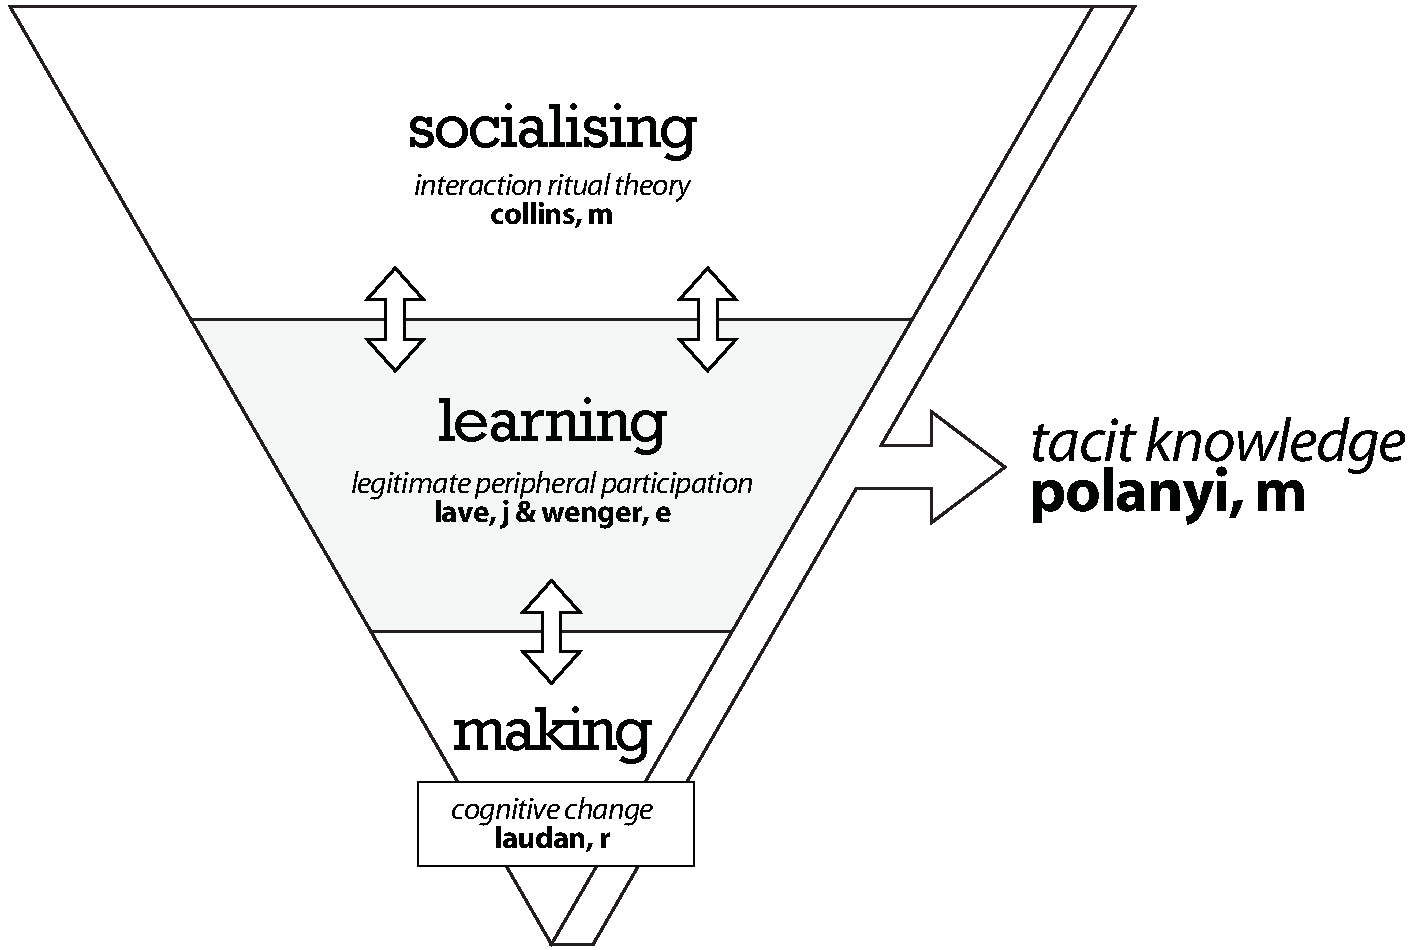
\includegraphics[scale=0.45,natwidth=10pt,natheight=1pt]{confirmation-report/graphs/pyramid01.pdf}
	\caption[Theoretical Relations]{Graphic relationship between theoretical approaches}
	\label{pyramid}
\end{figure}
%\end{center}

It is important to note that I do not see my three core chapters as independent, self-sustaining units. Rather, I regard their relation as a type of funnel-like structure or an inverted pyramid, going from broad to specific, from the everyday generalities of human contact to the much more unusual breakthroughs of value-adding innovation. Figure \ref{pyramid} aptly illustrates the reasoning behind the theoretical relations that will sustain the core of my dissertation, which have also heavily shaped my proposed methodological approach, described in more detail in section \ref{methodology}.

\newpage


 

\section{Thesis Structure}
\label{structure}

The macro-structure of my dissertation will be organised according to what \citet{dunleavy03} calls a ``compromise model'', emphasising the core research chapters (informally referred to as ``the beef'' by the author), without disregarding the always necessary lead-in chapters. Figure \ref{structure-graph} presents a schematic model of my proposed structure, detailing relative lengths of each chapter and macro sections with relation to the whole and providing a summarised view of each chapter.

%\begin{center}
\begin{figure}[ht]
	\centering
		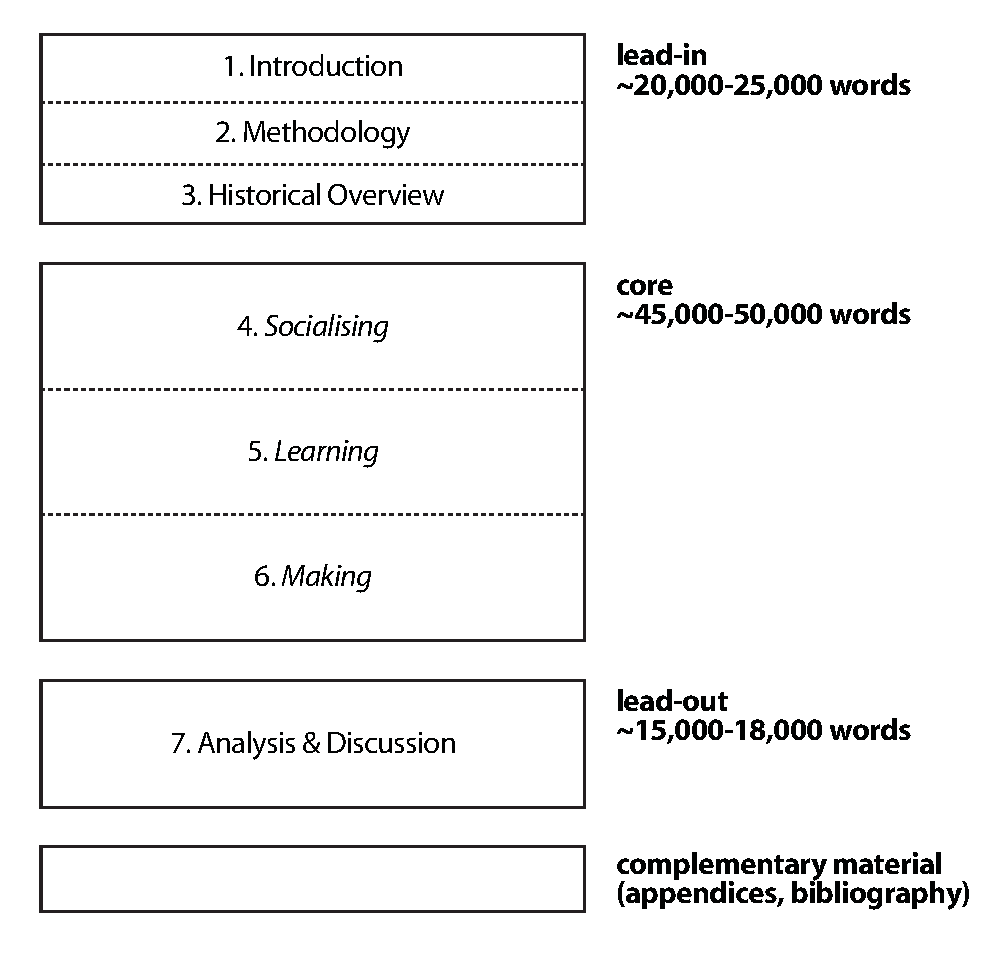
\includegraphics[scale=0.65,natwidth=10pt,natheight=1pt]{confirmation-report/graphs/structure01.pdf}
	\caption[Thesis Structure]{Theoretical structure of the dissertation's three core chapters}
	\label{structure-graph}
\end{figure}
%\end{center}


As mentioned above, the core of the dissertation will be divided into three chapters, each revolving around a different but complementary relationship and theoretical framework. Chapter 4, \textit{socialising}, will look at hackers' everyday rituals taking place inside hackerspaces using \citepos{collins04} interaction ritual theory. Chapter 5, \textit{learning}, will attempt to understand how social relations amongst hackers influence and facilitate their learning and transmission of technical skills. It will do so building upon \citepos{lave91} concepts of Legitimate Peripheral Participation and Communities of Practice. Further, Chapter 6, \textit{making} will seek to examine whether such skills can ultimately yield innovation in the form of valuable technological contributions. It will do so based upon \citepos{laudan84} model of Cognitive Change.

Present throughout the entire dissertation will be \citepos{polanyi66} concept of Tacit Knowing, attempting to make sense of the wider epistemological concern regarding the importance of physical presence in knowledge transmission. All three chapters will be supported by ethnographic data collected by means of participant observation and intensive interviewing in Melbourne, San Francisco and Bogot\'{a}.

Complementing the core macro section, chapter 2 will present a detailed account of the research design, the obtained data and a comprehensive rationale for each of the decisions made as a result of the research process. It will also attempt to report my experiences in the field: shortcomings, successes, rewards and any other eventualities. Chapter 3 will delve into the history of hackers and hackerspaces, providing much-needed context into the emergence of these communities and their members, whom I perceive as fitting into the wider category of Bohemia, all while reviewing existing scholarly literature.

Chapter 7 will provide a final analysis, discussing all findings from the perspective of tacit knowledge, examining the implications of such findings and, finally, linking them back to the existing literature, locating the contributions made by the work within its field of study.


%1. Brief intro
%2. Precedent
%3. Quick description of what the hole in the knowledge is
%4. How my thesis fits in there
%5. The Ethics hurdle
%6. Why ethnography?
%7. Subjects: hackers. why? start off by mentioning education in general and evolution of the project
%8. Field sites
	% ambitious
	% added complexity of multi-language
%9 Data
	% online data
	% frequency per week


\section{Research Methodology}
\label{methodology}

% Precedent

\subsection{Hacker Ethnography}

As a result of my background, I have interacted with hackers (of the free and open source software kind) on numerous occasions and moved naturally amongst them. As such, I believe my position is ideal for adopting an ethnographic approach ---one mostly consisting of fieldwork in the form of participant observation and complemented, at a narrower scale, by a reasonable number of qualitative interviews, as detailed below.

I see hackerspaces and the individuals who conform them both as a subcultural movement derived from the broader bohemian category and as communities of practice, sharing and fostering their skills and knowledge by virtue of their collective intellectual curiosity. In this context, I regard my choice of an ethnographic approach as suitable for a number of reasons. 

First, it will allow me to empirically test my hypotheses by allowing me to gain first-hand exposure to hackers and hackerspaces. Empirically obtained data is, in my case, essential, given the relative scarcity of scholarly works on hackerspaces. Second, it will then enable me to contrast my observations against my chosen framework and sub-frameworks and test for any theoretical inconsistencies that might arise, in search for what \citet{baszanger97} call a process of ``totalisation'' ---delineating their boundaries in accordance to the scope of my field. Third, ethnographic fieldwork will allow me to ``explore the tissue of [hackers'] everyday life to reveal the processes and meanings which undergird social action'' \citep[p.551]{herbert00}, that is, to gain an understanding of their social structure and in doing so, answering the puzzles formulated throughout this dissertation.

% Ethics hurdle

\subsection{Three Cities, Three Technoscapes, Three Hackerspaces}
\label{methods}

The growing presence of hackerspaces across the world poses an interesting challenge with regards to my methodological approach, the first of which is achieving a reasonable degree of what \citet{silverman00} calls \textit{generalisability} with regards to my findings, particularly when analysing a limited number of sites and given the budgetary constraints of a PhD candidate in lone-researcher mode\footnote{See section \ref{budget} for more on the financing of this project and solutions to budget constraints.}.

To address this issue, I will approach my fields with a globalised perspective, following \citepos{appadurai96} concept of \textit{scapes}, particularly, \textit{tech\-no\-scapes}:  irregular landscapes defined by the ``global and \ldots ever fluid configuration of technology'', attempting to make sense of the causes and effects such technology exerts within local, yet increasingly connected communities. I intend to adopt a centre-periphery approach, thereby choosing three specific hackerspaces in three different cities of the world, from San Francisco in the United States (centre) to Melbourne to Bogot\'{a}, Colombia (periphery). This choice is deliberate and the product of careful thought combined with my personal circumstances. Figure \ref{methodology_graph} provides a graphical representation of my selection as it fits into the research design detailed in this section.

\subsubsection{Half-way: \textit{Connected Community} in Melbourne}

I intend to undertake the greater part of my research in Melbourne, embarking in fieldwork at \textit{Connected Community}, the city's local hackerspace. Connected Community is a maturing space, with about 15 fee-paying members, over 40 collaborators\footnote{See \texttt{http://goo.gl/xaEUN}.} and a recently attained incorporation as a non profit organisation\footnote{See \texttt{http://goo.gl/dcUQk}.}.

Notwithstanding the fact that I am based in Melbourne, making it logistically convenient to adopt Connected Community as my main site, I see Connected Community as an ideal location for two main reasons. First, I regard it as being positioned half-way between the centre and the periphery of the hackerspaces technoscape, far enough from fully-developed technological foci, yet still within a developed nation with a relatively small but healthy IT landscape. As such, it will allow me to make cautious generalisations about the phenomenon, while also enabling me to corroborate and/or disprove most of my assumptions and to make the larger part of my observations long before embarking on costly travel overseas. Second ---and most important--- Connected Community is a community of practice in the making. Having recently formalised and incorporated but still being in its relative infancy, this hackerspace will provide me with a priceless opportunity to witness its evolution and growth, in terms of members, social relations and skills.

I intend to make Connected Community my primary field, performing the majority of my research with Melbourne-based hackers at their headquarters. This will allow me to have a strong frame of reference with which to make comparisons against technoscapes at the centre and periphery. Section \ref{strategy} delves into the research strategy in more detail.

%\begin{center}
\begin{figure}[ht]
	\centering
		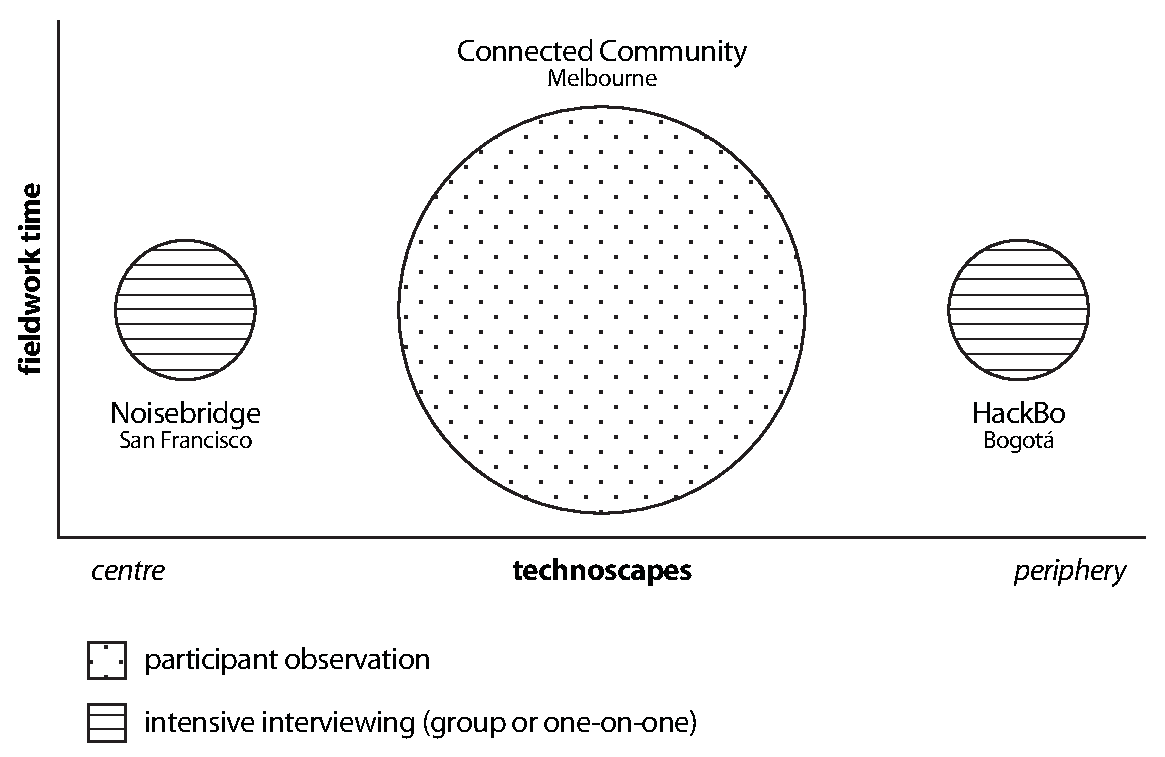
\includegraphics[scale=0.65,natwidth=10pt,natheight=1pt]{confirmation-report/graphs/methodology01.pdf}
	\caption[Synthesised Methodological Approach]{Synthesised methodological approach}
	\label{methodology_graph}
\end{figure}
%\end{center}


\subsubsection{Centre: \textit{Noisebridge} in San Francisco}

Noisebridge in San Francisco is one of the most prominent hackerspaces ---one that has served as a model for several others. Two main reasons make Noisebridge particularly noteworthy. First, it was one of the first original American spaces, founded by Mitch Altman, a well-known hacker who came up with the idea after his visit to the 2007 Chaos Communication Camp, a yearly hacker convention held in Germany\footnote{Section \ref{history} offers details on the conference's organisers: the Chaos Computer Club, a renowned hacker group.}. A piece on \textit{Wired} magazine details the genesis of Noisebridge, as well as American hackerspaces in general:

\begin{quote}
While many movements begin in obscurity, hackers are unanimous about the birth of U.S. hacker spaces (sic): August, 2007 when U.S. hackers Bre Pettis, Nicholas Farr, Mitch Altman and others visited Germany on a geeky field trip called Hackers on a Plane. \citep{tweney09}
\end{quote}

The second ---and most important reason for Noisebridge's notoriety is its location. As mentioned in section \ref{intro}, the origin of Silicon Valley as a central technological hub is closely tied to a group of early pioneers and the ever favourable influence of Stanford University and the U.S. Military \citep{lee00}. Today, and despite its well-known ups and downs, it is perhaps the most influential IT hub in the world, largely responsible for the technology-driven economic booms of the 1980s and 1990s in the United States \citep{bresnahan04}.

In curious contrast to this image of hi-tech behemoth, the Bay area at large has historically presented itself as a Mecca for countercultural movements at least since the 1950s, having served as base for the artists of the so-called \textit{San Francisco renaissance}, as well as becoming a centre for west coast beat poets, hippies, politically-aware students, radicals, dissidents, gays and a plethora of colourful characters.

Noisebridge's appeal thus lies in the fact that it is caught in the midst of the duality between the entrepreneurs and the bohemians: some of its members have long-standing careers in the Valley's tech industry, others have artistic or political backgrounds, while a special few seem to slide naturally between the two worlds. Altman himself is somewhat of a hippie and a pioneer of virtual reality technologies, having founded a company called 3ware\footnote{See \texttt{http://www.slideshare.net/maltman23}.}. Noisebridge's over 150 members range from professional programmers, to artists, activists and designers. It also has the dubious honour of counting Jacob Appelbaum (the most prominent American Wikileaks associate) as a founding member. Appelbaum has been the subject of several news reports lately, due to Wikileaks' spotlight, his relationship with Julian Assange \citep{rich10} and the continued harassment he has been subjected to by U.S. government officials \citep{mills10}.

\subsubsection{Periphery: \textit{HackBo} in Bogot\'{a}}

Some 6,000 kilometres south-east of San Francisco is HackBo, Bogot\'{a}'s own hackerspace. HackBo was founded in 2010 after three failed attempts to organise what was, until then, a loosely-tied community of mostly free and open source software hackers stemming from the country's public universities \citep{arizmendi11}. HackBo currently counts 15 fee-paying members and a larger number of associates\footnote{See \texttt{http://goo.gl/egzqK}.}, having now become a consolidated space, thanks in part to a strategic alliance with an already existing cultural centre, \textit{El Eje}\footnote{See \texttt{http://goo.gl/WXcTA}.} (The Axis), with which it shares a common habitat ---a house located in the city's university district. HackBo's members describe their space as an ``open community lab'' \citep{uribe11} where everybody is welcome to share their experiences and knowledge and to learn about computer languages and hardware hacking. 

HackBo was modelled after Hacker Dojo, another iconic American space founded by Lee Felsenstein\footnote{Felsenstein is a long-standing and well-known hacker, former moderator of the Homebrew Computer Club. See \citet{levy84} for more information.}. In terms of activities, it follows many of the same trends as other hackerspaces around the world: electronics tweaking, open source software and crafts, yet, for the purposes of my study, HackBo offers a very interesting opportunity.

Unlike the United States and Australia, whose budget for research and development is in the billions of dollars and represent relatively high percentages of their GDP\footnote{United States: 395.8 Billion, 2.8\% of GDP in 2010. Australia: 15.3 Billion, 1.8\% of GDP in 2010 \citep{wadsworth10}.}, Colombia occupies a humble fifty-second place, having invested about 600 million U.S. Dollars in 2007, only around .16\% of its GDP \citep[p.82]{unesco10}. Yet, there are perceivable cues that suggest change. Juan Manuel Santos, the recently elected President released an ambitious four-year plan for IT infrastructure immediately after reaching his position. The plan calls for an aggressive strategy to widen broadband usage and coverage in the country with special emphasis in depressed and remote regions, while promoting incentives for skills development and IT related business activities, particularly software development \citep{molano11}. 

Despite this ambitious push, which also includes the institution of three new IT research centres, there is still a relative scarcity of formal research entities in the country, a fact that raises the question as to whether or not hackerspaces can fulfil that role with some degree of success, either by positioning themselves as informal but effective research centres or by providing much-needed knowledge and skills to future researchers. 

Colombia's current stance with regards to ICT, combined with its unique cultural and social conditions, make HackBo attractive as a vehicle through which to study how environmental nuances influence learning and technological development inside hackerspaces.

\subsection{Research Strategy}
\label{strategy}

Ethnographic participant observation will be my primary research method, complemented by in-depth interviews at hackerspaces overseas. I intend to collect a substantial amount of data and to reach major preliminary conclusions before undertaking any research outside of Australia, the intention being to use interview data from overseas to test for representativeness and generalisability (as well as deviations) by contrasting it against the original, more comprehensive sample, hoping to verify and evaluate what should by then be a well-developed, yet early analysis.

I intend to spend a considerable amount of time amongst Melbourne hackers, assuming the role of a participant observer, regularly attending the Connected Community's weekly Tuesday meetings as well as some of the more informal weekend ``hang-out'' sessions. Tuesday meetings are of a formal nature and highly attended (thus ideal for performing Interaction Ritual Theory analysis), while the more spontaneous weekend meetups are somewhat more intimate and will hopefully provide insight into power relations, conflict and other intimate phenomena.

In attempting to work within the boundaries of my theoretical foundation, I have identified key elements on which to focus, hoping to find patterns and consistent behaviours that will subsequently lead to deep and hopefully fruitful analysis. While my intention is to gather data for all chapters in a concurrent manner, I will focus my observations sequentially in the same order as my three core chapters so as to build upon them as the work progresses. Outlined below are these main focal elements.

\subsubsection{Core 1: Applying Interaction Ritual Theory}

\begin{itemize}
  \item Identification of specific hacker rituals as well as their nature (formal, natural) and degree of success (successful, failed, empty, forced).
  \item Identification of ritual ingredients and outcomes in the context of hackerspaces --- \citet[p.41]{collins04} describes well-delineated causes and consequences of IRT. I will attempt to spot such factors in rituals held in hackerspaces, placing added emphasis in co-presence and barriers (ingredients) and symbols and negotiated morality (outcomes).
  \item Identification of key situations leading to ``symbolisation'' and the establishment of sacred objects.
\end{itemize}

\subsubsection{Core 2: Applying Legitimate Peripheral Participation}

\begin{itemize}
  \item Identification of a clear power structure in the context of LPP's examination of the duality between newcomers and old-timers and the prior analysis of IRT's sacred objects.
  \item Identification of instances of negotiated meaning and common concern. Similarly to Polanyi, \citeauthor{lave91} argue that knowledge is partly negotiated within a group. Within hackerspaces, analysis of this common meaning could be especially fertile, particularly in shedding light on the processes of learning and participation.
  \item Identification of motivation factors leading to the transition from peripheral to full participation within hackerspaces.
\end{itemize}

\subsubsection{Core 3: Applying Cognitive Change}

\begin{itemize}
  \item Identification of problem selection in the context of prior analysis of symbolisation (core 1) and negotiated meaning (core 2). Cognitive Change Theory places problem-solving at the centre of technological advance\footnote{It should be noted that the concept of problem-solving, according to the author, is indeed a broad one, involving not only ``utilitarian'' activities but also aesthetic and intellectual ones \citep[p.84]{laudan84}.}, thus the nature of problem selection becomes especially meaningful in understanding how technology flourishes in hackerspaces.
  \item Categorisation of types of problems solved by hackers within the CCT system.
  \item Identification of the effects of the ``environment'' as described by \citet[p.101]{laudan84} in relation to technological production in hackerspaces, considering prior analysis of settings and rituals. Also, identification of potential ``niche-isation'' in different hackerspaces and the determining factors in this process.
\end{itemize}

It is worth mentioning that I intend to conduct all my research overtly, with full disclosure to the community. I have already engaged some members of Connected Community at a personal level, yet all official data collection will begin only after gaining approval from the Monash University Human Research Ethics Committee (MUHREC). I should also note that I am already acquainted with the process of gaining ethics approval and performing research within the committee's guidelines as a result of having chosen similar methods for my Master's thesis. Section \ref{timeline} specifies my timeline for gaining ethics approval and undertaking participant observation at Connected Community.


\subsection{Data and Data Analysis}

Fieldwork at Connected Community in Melbourne will be documented primarily with the aid of fieldnotes, following \citepos{schatzman73} note-taking method. Summarily, the procedure involves labelling notes into three categories: Observational (ON), Theoretical (TN) and Methodological (MN). At a later stage, the notes are further categorised into logical thematic packages and complemented by analytic memos that serve as more explicit and elaborated theoretical notes. As noted earlier, my observations will take place overtly so I expect to be able to take ``jotted notes'' \citep[p.90]{lofland95} on the spot, transforming them to ``full fieldnotes'' at a later time. 

While fieldnotes seem to be the data-gathering method of choice for social scientists at large \citep{silverman00,lofland95,schatzman73}, I share \citepos{perakila97} concerns regarding their reliability. At best, fieldnotes provide a mediated account of events, filtered by the researcher's own points of view or interpretations. At worst, they can reflect erroneous observations and lead to mistaken conclusions. Thus, I will attempt to simultaneously collect raw data in the form of audio or video recordings to the extent to which such recordings are logistically, socially and ethically admissible.

For the purposes of interviewing, audio recordings alone will be the method of choice. Interviews conducted for my Master's thesis provided me with some methodological experience in conducting and logging sessions. My method involves taking carefully annotated notes prior to transcribing. Much like the fieldnote model described above, the notes are categorised and, more importantly, accompanied by a detailed, time-coded guide by which one can easily refer back to the original data.

Moreover, I seek to analyse all my qualitative data using \citepos{miles84} method, by means of three concurrent flows of activity: \textit{reduction}, whereby one selects, focuses and simplifies raw data, \textit{display}, involving assembling information so that it allows for ``conclusion drawing and action taking'' (matrices, graphs, networks) and \textit{conclusion/verification}, in which one connects causes and propositions in order to infer and determine. I realise that data coding can be an extremely laborious process, so my overall timeline for the completion of this project (see Section \ref{timeline}) accounts for these steps.

\subsection{Potential Woes}

Realising that there is no such thing as a perfect methodological design, or a one-size-fits-all solution, I consider the task of identifying potential shortcomings with the proposed research design a mission-critical one. This section attempts to provide preliminary reflections on potential shortcomings. It also offers possible solutions and/or counter-arguments.

\begin{list}{\labelitemi}{\leftmargin=0em}

\item[] \textbf{Familiarity with the setting}. While prior contact with hackers and relatively good knowledge about their social etiquette and practices is almost certainly a good thing, it also carries with it the risk of making the researcher ``feel too comfortable''. \citet{hammersley90}, seems to agree by arguing that ``when a setting is too familiar, the danger of misunderstanding it is especially great''. It is thus important not to take anything for granted and to attempt to disregard previous facts or assumptions that are the result of prior experience. As such, making a conscious effort to enter the field without any biases or preconceptions is crucial.

Under this same category, one can find the risk of developing over-rapport with research subjects. Familiarity and shared values can stop a researcher from evaluating his or her settings critically. Establishing rapport is an ever-present recommendation in fieldwork guides, yet the risk of over-sympathising with members of the communities under study can result in lack of critical judgement. On the topic, \citet{roberts94} asks: ``how does one, whose self interests are foremost in beginning an examination of a social world, hope to remain objective enough to command a claim of validity from his audience?''. I do not believe there is a straightforward answer to that question, yet I am convinced that active and deliberate steps must be taken in order to prevent the loss of a researcher's independence and capacity for critical inquiry.

\item[] \textbf{Under-analysis of data}. Having chosen to study multiple fields, I run the risk of either collecting too much or too little data for any one of them. I have considered this possibility and attempted to minimise it by selecting specific (and meaningful) events to assist to while performing participant observation in Melbourne. With that same frame of mind, I have decided to limit fieldwork for my other two sites so as to only seek to identify similarities and divergences from tendencies already observed in Melbourne. This will hopefully provide me with a reasonable volume of data ---one that aids in reaching accurate findings without becoming overwhelming. Needless to say, this potential catch will also be considered when determining the number of interviews to be conducted at the two hackerspaces overseas.

\item[] \textbf{Multiple methods} \citeauthor{silverman00} warns about possible complications stemming from the use of multiple research methods: ``multiple methods may tempt novice researchers to move to another dataset when they are having difficulties in analysing one set of material'' \citep[p.134]{silverman00}. I share the author's concern, yet I view my methods as complementary. In essence, I will avoid turning to one set of data when the other does not fit. Instead, I will only use interview data to explicitly contrast existing findings that are the product of previous fieldwork in Melbourne.

\end{list}

By identifying potential problems with my methodology before they happen, I aim to minimise their impact and to plan out possible solutions or alternative methods if needed. I consider this section to be nothing more than a work in progress, in the sense that the above list will be extended, developed and revised as this work moves forward. 


\subsection{Some Thoughts on Financing and Logistics}
\label{budget}

This project is, by design, ambitious in nature. Not only is it broad in scope, but it also considers fields separated by great distances. As exciting as this sounds, its logistics can indeed become a cause for concern for a single PhD candidate with a moderate budget. Thus, securing proper financing has become an on-going priority. 

I intend to apply for a Postgraduate Travel Grant to conduct fieldwork\footnote{See \texttt{http://goo.gl/OwtyD}.}. As mentioned in section \ref{methods}, my choices of overseas hackerspaces have also been shaped by my personal circumstances. I am a Colombian citizen from Bogot\'{a}. I have been acquainted with various members of the hacker community in that city for a number of years and personally know at least one of the members of HackBo. This will reduce my barriers of entry to the site in terms of time and resources, while allowing me to cut my travel expenses by having a place to stay while I conduct my research. Moreover, due to the nature of international flight hubs, the simplest, most cost-effective way for me to fly to Bogot\'{a} is by connecting flights at the Los Angeles Airport in California. As a result, the logistics of my research at Noisebridge will be greatly minimised, as my stay in San Francisco will be relatively simple to arrange.

In light of the fact that time spent overseas will be short, I cannot engage in the same type of long-term participant observation I intend to conduct in Melbourne. Consequently, I have opted to adopt intensive interviewing as my main research method at these locations. Much like \citet{lofland95}, I do not view intensive interviewing as a substitute for participant observation. Rather, I see both methods as being complementary and appropriate for each of my circumstances, as I intend to build upon previous findings at these locations.

Naturally, much if not all of the preparatory work for these interviews will take place in Melbourne. I intend to contact members of both hackerspaces immediately after gaining ethics approval, well in advance of my trip. Having been a subscriber to both Noisebridge's and HackBo's public email lists since December 2010, I expect to be able to identify key members and to approach them prior to reaching my destinations.



%Furthermore, fieldwork will draw upon the work of burrell09, who views the ethnographic field as a ``cultural network'' composed of ``spaces, people and objects'' [p.189]burrell09 made up of multiple sites (some physical, some mediated) that ultimately converge into a single unit, much like \citepos{appadurai96} multiple \textit{scapes} represent a single cultural flow or Manuel Castells' view that ``society'' and ``network'' are increasingly fusing [p.65]lovink03.


\section{Writing samples}
\label{samples}

Please note that these two samples are taken out of a wider context. They should be understood not as whole logical units but rather as parts of two separate subchapters inside which they make more sense. The two subchapters from which these samples are taken are gladly available if needed.

\subsection{Sample 1: Hacker Origins and Philosophy}
\label{history}

The tradition of hacking has its origins within a formal academic environment. Indeed, the word ``hacker'' as a descriptor of the creative, technologi\-cal\-ly-savvy and computer enthusiasts first came into use at the Massachusetts Institute of Technology, where it derived from the older tradition of harmless and ingenious pranks some students devised (and still devise) at the University's campus \citep{levy84}\footnote{\textit{Hacking}, in this context, is a wonderful MIT tradition whereby students come up with elaborate jokes that demonstrate their technical prowess as well as their sense of humour. One example of a memorable hack was the placement of a police car on the top of the Institute's \textit{Great Dome}. For a full list of hacks, see \texttt{http://hacks.mit.edu/}.}.

As a result of the media's adoption of the term as a synonym for computer criminals, academic use of the word is heterogeneous at best and discordant at worst. Some scholars and researchers in the field of information technology and computer security have chosen to follow the media's trend, using the term to describe malicious computer users, thus making literature on the subculture that originated at MIT in the late 1950s extremely difficult to distinguish. In his book \textit{Hacker Culture}, author Douglas Thomas \citeyearpar{thomas02} takes a rather neutral stand on the etymological divergences of the word, choosing instead to focus on the consequences of such divergences: ``the very definition of the term `hacker' is widely and fiercely disputed by both critics and participants in the computer underground'', a fact that, in his view, ``gives a clue to both the significance and the mercurial nature of the subculture itself''. Such eclectic positions, however, add an additional layer of complexity to the task of performing a thorough literature review on \textit{any} of the word's conveyed meanings.

Indeed, the concept of hackers as a collective is as filled with almost as many contradictions as the word itself. While it would be easy to classify them into the formal side of Theodore Roszak's \citeyearpar{roszak69} radical cultural division of the post-war years, as members of a closed inner circle, or a techno-elite, I set out to prove that, in fact, hackers are quite the opposite, having more in common with Roszak's concept of counter-culture (which, as shall be discussed, is composed of many heterogeneous groups). Other scholars, such as McKenzie Wark \citeyearpar{wark04} have gone as far as comparing hackers to Marx's concept of the \textit{proletariat} ---presenting them as the exploited class of the information age.

Steven Levy's \textit{Hackers: Heroes of the Computer Revolution} \citeyearpar{levy84} is widely recognised as a fundamental, landmark piece of literature when it comes to historically documenting the emergence of the original hackers as an identifiable group and subculture. While not academic in nature, Levy's work can not only be considered an obligatory reference but also a document of historical significance itself, having provided an initial written declaration of philosophical principles, to which he dedicated an entire chapter of his book. Levy described what he called `The Hacker Ethic' ---a set of undeclared maxims that seemed to have originated along with the genesis of the movement, when the very first hackers lurked building 26 at MIT, hoping to harness unused, idle time from one of the first (and quite primitive) computers ever assembled:

% In the mid-’80s, following a rash of computer break-ins by teenagers with personal computers, true hackers stood by in horror as the general public began to equate the word — their word — with people who used computers not as instruments of innovation and creation but as tools of thievery and surveillance levy2010


\begin{quotation}
\ldots the dozen or so hackers were reluctant to acknowledge that their tiny society, on intimate terms with [the computer], had been slowly and implicitly piecing together a body of concepts, beliefs and mores.

The precepts of this revolutionary Hacker Ethic were not so much debated as silently agreed upon. No manifestos were issued. No missionaries tried to gather converts.
\end{quotation}

\noindent
If not the first, Levy was certainly amongst the earliest of theorists who saw the necessity to explicitly declare those ``concepts, beliefs and mores'', which he dubbed \textit{The Hacker Ethic}, consisting of six initial precepts:

\begin{enumerate}
\item Access to computers ---and anything which might teach you something about the way the world works--- should be unlimited and total. Always yield to the Hands-On Imperative!
\item All information should be free
\item Mistrust Authority - Promote Decentralization
\item Hackers should be judged by their hacking, not bogus criteria such as degrees, age, race or position
\item You can create art and beauty in a computer
\item Computers can change your life for the better
\end{enumerate}

\noindent
Inherent in such principles were ideas of freedom of information, anti-establishment and outright technological determinism, most of which remain unchanged to this day. Levy's precepts provide a clear, coherent basis to perform an analytical dissection of the emergence of the hacker movement. Precepts 1 and 2 summarise the movement's views on issues of freedom of information and their discrepancies with increasing restrictions on copyright and patent law, particularly for software but increasingly towards other types of ideas and works. Hackers were born within ---and still share close ties to--- an academic environment. Across the world, universities and academic institutions still foster and cherish the sharing of information. Gift economies are prevalent amongst academics, who continually build upon each other's work and who, just like those first hackers, are flattered ---not threatened--- to see others use and expand their own work.

Precepts 3 to 5 present an interesting perspective on Hackers' world-views, particularly when it comes to their relation with the wider spectrum of society. By making a personal interpretation of these three principles, I conclude that today's Hackers are heirs to the wider bohemian tradition that began in Europe during the 19th Century and subsequently evolved into the 1960s and 1970s counter-cultural movements, with which they shared similar views, tastes and political ideas.

Lastly, I judge the last precept to represent a growing trend towards technological determinism, reflective of the growing view that human and social development are closely tied to the advance of technology. 
%insert very very brief intro to tech determinism


\subsection{Sample 2: The Many Implications of Polanyi's Epistemology}
\label{polanyi}

The transmission of certain skills and knowledge, argued Michael Polanyi, requires a cooperative process of dialogue and unspoken understanding made possible by human contact through physical proximity, interaction and a certain degree of cultural affinity. Of course, this postulate is not new. Since Plato (and perhaps earlier), philosophers have identified a human dimension involved in learning. Polanyi's angle, however, is unique in a number of ways. Indeed, to fully apprehend it, one must examine these within a historical frame.

First, Polanyi dared to challenge a prevailing epistemological paradigm, (referred to as ``the objective ideal'') that became prevalent as a result of the ``scientific triumphs'' \citep[p.17]{gelwick77} that took place after the Copernican revolution but the causes of which began far earlier, with several historical developments that were, in his view, instrumental in leading to it.

Amongst them was the gradually increasing tension between two concepts he described as moral scepticism and moral perfectionism. From Greece onwards, the phenomenalist view that moral knowledge was unat\-tainable continued and grew in the works of modern thinkers and philosophers such as the Marquis de Sade, Nietzche and Rimbaud. Modern existentialism, Polanyi argued, uses moral scepticism to attack social morality as artificial and hypocritical. This progressive devaluation of moral values, however, could not by itself sway society on its way towards the mass adoption of the objective ideal: the degradation of judeo-christian morality caused partly by the advent of scientific rationalism led some to pursue such values even more passionately. Attacks on christianity during the Enlightenment led to the transposition of moralistic dogmas away from religion and ``into man's secular thoughts'' \citep[p.57]{polanyi66}, thus creating a strange collision between the rationality and objectivity sought by the nascent enlightened society with a secularised moral demand for social improvement. 

While Polanyi conceded that this tension initially led to the improvement of ``almost every human relationship, both private and public'', he also claimed that the increasing radicalisation of these views not only posed ``dangerous internal contradictions'' \citep[p.58]{polanyi66} but had led to the rise of existentialism, nihilism and further, Marxism, the tragic result being the discredit of ``all explicit expressions of morality''. The tension between the two sides, thus, resulted in a ``paradox of morality'' which ultimately led modern society to seek solace in absolute and almost thoughtless objectivity.

Second in the set of consequences leading to the wide adoption of the objective ideal (and the dawn of the ``modern scientific revolution'') was, according to Polanyi, the mechanisation of society. By means of a simple but eloquent account of the process leading to the growth of mechanism, he discussed this point with a brief historic recount, starting from Greek times, specifically Pythagoras, who came to view the world ``exclusively in terms of numbers''. Numerical relationships as beautiful as those found within triangles, thought Pythagoras, were present in all aspects of the world. Post Copernicus (and even more so after Kepler) the universe came to be seen as a mechanical system running with clock-work precision ---a fact that delighted those who studied it. \citet[p.7]{polanyi58} noted that Kepler regarded his own discoveries in ``ecstatic communion'', amazed and bewildered by the universal precision found in god's creation. Yet, after Galileo and Newton, things changed. Rather than being an inherent universal force, mathematics went on to be regarded simply as a summary of experience:

\begin{quote}
Numbers and geometrical forms are no longer assumed to be inherent as such in Nature. Theory no longer reveals perfection; it no longer contemplates the harmonies of Creation \ldots `pure' mathematics, formerly the key to nature's mysteries, became strictly separated from the \emph{application} of mathematics to the formulation of empirical laws. \citep[p.28]{polanyi58}
\end{quote}

What was to follow would be an almost inevitable progression from Descartes' rationalism to zealous objectivity marked the decline of the Enlightenment and the dawn of Mechanism, as proclaimed by many voices, the loudest of which was that of Ernst Mach, from the Vienna school of positivism and his book \textit{Die Mechanik}, published in 1883. 

It was to be Polanyi, then, who would restore confidence in human intuition by demonstrating an ever-present human element intrinsic in the act of knowing:

\begin{quote}
Both a craftsman and a novice are capable of identifying a particular tool and indicating some of its functions, but what distinguishes the craftsman's knowledge from that of the novice lies in the former's ability to use the tool subsidiarily in order to focus on the object of his craft. In the case of the scientist, he is not only identified by his explicit knowledge of given premises, but by his subsidiary utilization of those premises in the practice of science \citep[pp23-24]{kane84}.
\end{quote}

This analogy is particularly enlightening in the sense that it illustrates how Polanyi's thesis has extensive implications within today's prevailing systems for the acquisition of knowledge. Polanyi's unusual career pathway ---from the exact sciences to sociology and philosophy--- made him acutely aware of the need to ground his precepts on modern foundations, applicable to and compatible with modern practices and standard conventions of generally accepted scientific practices. Indeed, it was the scientific process itself that he sought to reform, for he reckoned that its very conception relied on principles which were ignored and sometimes expressly denied by many of his colleagues. 

Polanyi understood that no scientific theory can (nor should it) achieve perfect objectivity. As such, the boundaries of knowledge are ever broadened by reliance on certain presuppositions ---sets of which he dubbed ``subsidiary knowledge'', reached by using the senses as ``clues'': vehicles through which one can transcend into more abstract realms that ultimately lead to the acquisition of focal awareness or focal knowledge. Both types of awarenesses ---focal and subsidiary--- are necessary for new knowledge to occur.

Each new discovery (acquisition of explicit knowledge) is accompanied by a number of ``premises'' which do not (and cannot) stand on their own and that, until proven, remain as tacit or a-critical pieces of subsidiary awareness. Yet, they are essential to broadening the boundaries of scientific comprehension. Polanyi judged the almost obsessive scientific strive for objectivity to be misguided, arguing that all aspects of scientific discovery: data, theory and experimentation relied not only on said unproven subsidiary knowledge but also on the personal interpretation of these elements. Polanyi described these ``premises'' as by-products of proven theories ---by becoming proven themselves, they move into the realm of the explicit. If they are disproved, though, they are replaced, often generating Kuhn-style paradigm shifts.

In making such bold affirmations, however, Polanyi ran into an apparent dilemma, as, at first glance, it would sound like a recipe for the advocacy of blind faith and/or the lenient type of ``science'' practised by fanatics and supporters of pseudo-scientific belief systems. Indeed, insofar as personal interpretation (or subjectivity) is regarded as an integral part of the scientific method, all claims, including unsubstantiated or even fraudulent ones, would gain an aura of validity which would, very rapidly, over-flood the gates of serious inquiry to the point where it would ``run the risk of discontinuity and ultimately, inertia'' \citep[p.37]{kane84}. 

As a consummate and respected scientist, Polanyi was firmly committed to the rigorous experimental techniques of accepted scientific practices and intimately familiar with their minutiae, virtues and flaws. Consequently he was perfectly aware of this apparent predicament, which he addressed by means of the application of a concept he dubbed the ``conviviality of science'' whereby said gates are guarded by scientific communities, bound together by common thought, solid standards, deep tradition and a desire for accuracy and rectitude\footnote{One could replace these last two concepts with, simply, ``the truth''. However, keeping with Polanyi's canons an absolute concept such as truth does not do the point presented any favours.}. 

Ever the scientist, Polanyi sought to improve the act of knowing by correctly identifying its idiosyncrasies, a fact that marks the second particular aspect that differentiates his epistemological system from preceding ones also considering a human element, as it is grounded on present-day reasoning and meant to aid understanding and resolving the present-day problems associated with the acquisition of knowledge: ``man can transcend his own subjectivity by striving passionately to fulfil his personal obligations to universal standards'' \citep[p.4]{polanyi58}.

A third aspect differentiating Polanyi's theory from earlier ones is its advocacy for strong independence as a necessary condition for the production and transmission of knowledge. Polanyi recounts his conversations with a ``leading communist theoretician'' by the name of Bukharin\footnote{We assume that Polanyi refers to Nikolai Bukharin, a	 Soviet politician executed by Stalin in 1938.} \citep{polanyi66}, who argued that pure research ---\textit{scientia gratia scientis}--- was ``a morbid symptom of class society''. Polanyi was appalled by Bukharin's appraisal, which he saw as a reflection of what he considered to be an over-mechanised and utilitarian society, where express and useful purpose was required for all endeavours, including the pursuit of knowledge. Relegating research activities to central control, he argued, significantly decreased their effectiveness, as a certain degree of flexibility vastly improves the success of epistemological ventures. Communism had no room for the type of serendipitous discoveries that lead Pasteur to give birth to the field of immunology and Flemming to discover Penicillin.

Polanyi viewed state-controlled science as an early warning of the advent and growth of totalitarianism across Europe, pre World War II \citep{polanyi36}. By committing to central plans in the pursuit of knowledge, ``thinkers'' (scientists, scholars, intellectuals) relinquished their power to contradict the powerful by appealing to the truth. Judging by what was to become the immediate political state of Europe, Polanyi's arguments proved to be eerily accurate.


%

\section{Coming of Age of a Subculture}



At first glance, a clear evolutionary link between the hacker subculture and bohemians, as first described in the early 19th Century is dim. In studying the history of Australia's bohemian tradition, Tony Moore \citeyearpar{moore07} analysed the relationship between 19th Century-style bohemians and the multitude of subcultural and countercultural movements born with the generation of baby boomers, from the late 1950s on. While technologically-minded hackers may be at odds with \citepos{roszak69} critique of the state of the society he lived in, which he described as being a harmful, or rather, dulling \textit{technocracy}, many of the bohemian traits identified by Moore seem as compatible with the early MIT hacker ethos as they were with those of the writers, artists and activists that inherited the values and customs of the bohemian legacy. In this chapter I argue that hackers are indeed unlikely heirs of that legacy too. I also analyse how the nuances and cultural traits of their origins manifest in the present, leading to the origin of modern-day hackerspaces.

\label{history}
\subsection{Hacker Origins and Philosophy}

The tradition of hacking has its origins within a formal academic environment. Indeed, the word ``hacker'' as a descriptor of the creative, technologi\-cal\-ly-savvy and computer enthusiasts first became used at the Mas\-sa\-chu\-setts Institute of Technology, where it derived from the older tradition of harmless and ingenious pranks some students devised (and still devise) at the University's campus \citep{levy84}\footnote{\textit{Hacking}, in this context, is a wonderful MIT tradition whereby students come up with elaborate jokes that demonstrate their technical prowess as well as their sense of humour. One example of a memorable hack was the placement of a police car on the top of the Institute's \textit{Great Dome}. For a full list of hacks, see \texttt{http://hacks.mit.edu/}.}.

As a result of the media-fuelled adoption of the term as a synonym for computer criminal, its meaning within academic boundaries is heterogeneous at best and discordant at worst. Some scholars and researchers in the field of information technology and computer security have chosen to follow the media's trend, using the term to allude to malicious cyber-intruders, thus making literature on the subculture that originated at MIT in the late 1950s extremely difficult to distinguish.

In his book \textit{Hacker Culture}, author Douglas Thomas \citeyearpar{thomas02} takes a rather neutral stance on the etymological divergences of the word, choosing instead to focus on the consequences of such divergences: ``the very definition of the term `hacker' is widely and fiercely disputed by both critics and participants in the computer underground''. In his view, this ``gives a clue to both the significance and the mercurial nature of the subculture itself''. Such eclectic positions, however, add an additional layer of complexity to the task of performing a thorough literature review on \textit{any} of the word's conveyed meanings.

Indeed, the concept of hackers as a collective is filled with almost as many contradictions as the word itself. While it would be easy to place them on the more formal side of Theodore Roszak's \citeyearpar{roszak69} cultural division of the post-war years, as members of a closed inner circle, or, more aptly, a techno-elite, I aim to prove that, in fact, hackers are quite the opposite, having more in common with Roszak's counterculture. Other scholars, such as McKenzie Wark \citeyearpar{wark04} have gone as far as describing hackers as a digital age Marx-style \textit{proletariat} where ``vectiorialists'' (capitalists) control and exploit their labour and profit from it.

Steven Levy's \textit{Hackers: Heroes of the Computer Revolution} \citeyearpar{levy84} is widely recognised as a fundamental, landmark piece of literature when it comes to historically documenting the emergence of the original hackers as an identifiable group and subculture. While not academic in nature, Levy's work can not only be considered an obligatory reference but also a document of historical significance itself, having provided an initial written declaration of philosophical principles, to which he dedicated an entire chapter of his book. Levy coined the term `The Hacker Ethic' to describe set of undeclared maxims that seemed to have originated in parallel with the movement itself, when early hackers lurked building 26 at MIT, hoping to harness unused, idle time from one of the first (and very primitive) computers ever assembled:

% In the mid-’80s, following a rash of computer break-ins by teenagers with personal computers, true hackers stood by in horror as the general public began to equate the word — their word — with people who used computers not as instruments of innovation and creation but as tools of thievery and surveillance levy2010


\begin{quotation}
``\ldots the dozen or so hackers were reluctant to acknowledge that their tiny society, on intimate terms with [the computer], had been slowly and implicitly piecing together a body of concepts, beliefs and mores.

The precepts of this revolutionary Hacker Ethic were not so much debated as silently agreed upon. No manifestos were issued. No missionaries tried to gather converts.''
\end{quotation}

\noindent
If not the first, Levy was certainly amongst the earliest theorists who saw the necessity to explicitly declare those ``concepts, beliefs and mores'', \textit{The Hacker Ethic}, consisting of six precepts:

\begin{enumerate}
\item Access to computers ---and anything which might teach you something about the way the world works--- should be unlimited and total. Always yield to the Hands-On Imperative!
\item All information should be free
\item Mistrust Authority - Promote Decentralization
\item Hackers should be judged by their hacking, not bogus criteria such as degrees, age, race or position
\item You can create art and beauty in a computer
\item Computers can change your life for the better
\end{enumerate}

\noindent
Inherent in such principles were ideas of freedom of information, contempt for the establishment and technological determinism. I suggest that the Hacker Ethic provides a clear, coherent basis upon which to perform an analytical dissection of the emergence of the hacker movement. Precepts 1 and 2 summarise the movement's views on issues of freedom, with an emphasis on information as well as their opposition to restrictions imposed by copyright and patent law.

Hackers were born within ---and still share close ties to--- academia. Across the world, universities still foster and cherish the sharing of information. Gift economies are prevalent amongst academics, who continually build upon each other's work and who, just like those first hackers, are flattered ---not threatened--- to see others use and expand their own work.

Precepts 3 to 5 present an interesting perspective on Hackers' world-views, particularly when it comes to their relation with the wider spectrum of society. By making a personal interpretation of these three principles, I conclude that today's Hackers are heirs to the wider bohemian tradition that begun in Europe during the 19th Century and subsequently evolved into the 1960s and 1970s countercultural movements, with which they shared similar views, tastes and political ideas.

Lastly, I judge the sixth precept to represent a growing trend towards technological determinism, reflective of the growing view that human and social development are closely tied to the advance of technology. 
%insert very very brief intro to tech determinism and comment out for paper


\subsection{Heirs of the Bohemian Tradition}

% --------------------------------------
% SUBINDEX
% --------------------------------------

% 1. Multiplicity of countercultures
% 2. Denial or contempt for the establishment
% 3. Criminal label & other carnivalesque traits
% 4. Geeks and Nerds
% 5. Position towards commercialism and capitalism
% 6. Nostalgia




% --------------------------------------
% Begin subsection
% --------------------------------------


% % 1. Multiplicity of countercultures
\subsubsection{One Counterculture, Many Subcultures}


In 1969, Theodore Roszak described the growing rebelliousness of the baby boomer generation as a \textit{counter-culture}: ``a culture so radically disaffiliated from the mainstream assumptions of our society that it scarcely looks to many as a culture at all, but takes on the alarming appearance of a barbaric intrusion''. Such disaffiliation was certainly not new: 19th Century bohemians (and others before them) already held many of the social grievances described by Roszac. It was, however, the sheer scale of the new movements ---strengthened in numbers by the offspring of couples formed in the post-war years--- that made the 1960s manifestations particularly powerful, even if, in reality, most of those movements were heterogeneous in nature.

As argued by various scholars \citep{mcgregor75,spates76,eder90}, a single, uniform counterculture as proposed by \citeauthor{roszak69} was nothing more than a gross generalisation. \citet[p.148]{hebdige87} further argued that the term came to represent an ``amalgam of
`alternative' middle-class youth cultures'' in macro-political opposition to what has been called the ``the establishment'', ``straight society'' or simply, ``the mainstream''. Yet others, like \citet[p.87--88]{marchant03} have criticised this view as over simplifying.

In this context, I take a practical approach and view individual movements as different, specific subcultures, all of which are enclaved in a countercultural social scope. Therefore, as eclectic as such groups were, opposition (whether backed by micro or macro-political action) was indeed their strongest bond. In this sense, hackers, bohemians, students and hippies were no different. As will be argued, such disdain for established traditions, authorities and the prevailing social order offered them empowerment yet came with a sense of irony, as many of the movements (hackers included) were born either inside or as a result of established institutions. Hackers' genesis, for instance, took place inside universities and in many cases with the financial and technical support of much-loathed institutions like the U.S. Department of Defence.

% ****************************************
% This is where the clarification on the
% issue of subculture/counterculture needs
% to go. Get subcultural reader
% ****************************************



% 2. Denial or contempt for the establishment

\subsubsection{Contempt for the Establishment}

Despite this element of irony, denial of established values, institutions and customs became the driving force for the self-identification of all movements of the time. In his Doctoral Thesis, Tony Moore examined the cultural \textit{status quo} that bohemians before them both challenged and benefited from:

\begin{quote}
\ldots bohemians performed publicly an imagined or hoped for personal autonomy from art markets that involved style, behaviour, art, social formations and even politics that transgressed and subverted, \emph{but never overturned}, bourgeois society \citep[p.10]{moore07}. [emphasis added]
\end{quote}

\noindent

By publicly expressing contempt for that society and positioning themselves as social outsiders, such characters ---who had long before acquired a sense of group identity--- managed to leverage a sense of ``forbidden fascination'' exerted in the wider social strata by means of ``coded fashion and recreation that could be read by the initiated'' \citep[p.17]{moore07}. Upon the dawn of the 1960s movements, such codes were further disseminated and strengthened by the powerful effects of the mass media.

As political awareness increasingly grew amongst many subcultural movements, condemnation of mainstream values became not only more outspoken but action-driven, shifting from a rather tolerant acceptance of the prevailing \textit{status-quo} towards a more politicised resistance that culminated in the protests of May of 1968 in France, the violent, anti-Vi\-et\-nam intervention demonstrations in university campuses across North America and the radicalisation of many movements across Latin America, where the very real possibility of the overturning of bourgeois society spurred revolutions and dictatorships whose consequences are felt to this day.

Drawing parallels between these events and the emergence of hackerism is not a simple task ---one not made any less complicated by the fact that the amount of scholarly works on the subject is rather modest, particularly when compared to other movements of the time. The limited amount of resources available nevertheless sheds some light on the issue of hackers' analogous disdain for established orders. \citet{levy84}, for instance, provided a sound starting point with his Hacker Ethic. The third maxim, ``Mistrust authority. Promote decentralization'', sheds extra light on the link between hackers and the wider countercultural spectrum.

This link becomes clearer by examining the history of the dawn of hackers, whose rhetoric, like that of many other movements of the time, became increasingly politicised during the 1960s and 1970s. Hackers imagined a world ``where computers would lead the way to a new, liberating lifestyle'' \citep[p.168]{levy84}. Much like other movements, they envisioned a way out of the social constraints of society, yet did so in their own, unique way, believing computers to be the main vehicle with which to achieve this.

In addition, \textit{Hackers} bluntly documents behaviour that is quite contrary to Roszak's concept of ``technocracy''. MIT hackers, Levy argued strongly, held passionate and vocal disdain for Weber-style bureaucracy. The focus of such disdain was inevitably embodied by International Business Machines (IBM) ---the devil they knew best, and later by countless more companies as well as the corporate culture they seemed to represent. In describing hackers' loathing for IBM types, Levy commented:

\begin{quote}
All you had to do was look at someone in the IBM world, and note the button-down white shirt, the neatly pinned black tie, the hair carefully held in place, and the tray of punchcards in hand. \citep[p.42]{levy84}
\end{quote}

Interestingly, this exact same stereotype is referenced by Roszak in his book. Upon discussing the nature of ``grown-upness'' he describes countercultural youth as having ``better ideas than GM or IBM seem able to offer'', describing them as a ``scruffy, uncouth, and often half-mad lot'' \citep[p.32]{roszak69}. Hackers' choice of clothes and odd sense of style thus followed a conscious effort to distance themselves from the formality of the corporate environment, embodied by the stereotype of the IBM employee, in the same sense as hippies and others rebelled themselves by opposing the idiosyncrasies and fashions of 1950s suburban America \citep[p.34]{heath05}. Their anti-establishment sentiments differed, however, in one fundamental way when compared to those of other subcultural groups of the time: their inherent motivations.

Beats, hippies and even anti-war protesters' unease seemed to stem from evolving views on Marxist and Freudian theories. Countercultural interpretations of Freud saw culture, or rather, civilisation as a sort of straitjacket constraining individuality and freedom \citep{heath05}. Hackers instead viewed individual freedom as achievable \emph{through} the more pressing matter of freedom of information. Thus, just as individuality was crucial for the development of group identity and sense of belonging in the case of the former, freedom of information became hackers' foremost foundational dogma. In practice, no single subculture would have thrived in its absence.



% 3. Criminal label & other carnivalesque traits

\subsubsection{The Criminal and the Carnivalesque}

Hackers are curious by nature. They satisfy their curiosity by engaging in acts of discovery, whether that means solving a problem or deciphering the inner workings of a machine or network. While, every so often, a hacker may break the law, there seems to be a wide mis-representation of hackers ---true hackers--- as criminals. This negative connotation has its origins some time in the 1980s. Richard Stallman \citeyearpar{stallman02b} explains: 

\begin{quote}

\ldots when I say I am a hacker, people often think I am making a naughty admission, presenting myself specifically as a security breaker. How did this confusion develop?

Around 1980, when the news media took notice of hackers, they fixated on one narrow aspect of real hacking: the security breaking which some hackers occasionally did. They ignored all the rest of hacking, and took the term to mean breaking security, no more and no less. The media have since spread that definition, disregarding our attempts to correct them. As a result, most people have a mistaken idea of what we hackers actually do and what we think.

\end{quote}

While the media may have been responsible for spreading the negative connotation, validation for the practice seems to have been the result of the publishing of three landmark books about computer criminals \citep[p.xiii]{thomas02}. Katie Hafner and John Markoff's \textit{Cyberpunk} \citeyearpar{hafner91}, William Gibson's iconic novel, \textit{Neuromancer} \citeyearpar{gibson84} and Clifford Stoll's \textit{The Cuckoo's Egg} \citeyearpar{stoll89}. All three books referred to their characters as ``hackers'', making little effort to draw a clear semantic distinction between their respective characters (real and fictional) and the wider hacker subculture. 

Stoll, a scholar, mathematician and astrophysicist, proficient in several computer languages and technologies was aware of the emerging trend and the irritation it caused amongst self-confessed hackers, yet chose to follow it. ``A computer wizard?'', he asked sarcastically at the beginning of his book. ``Not me ---I'm an astronomer'' \citep[p. 1]{stoll89}.

Perhaps as a wilful effort to appease the outcry, Stoll justified his decision with an apologetic opening paragraph:

\begin{quote}
What word describes someone who breaks into computers? Old style software wizards are proud to be called hackers and resent the scofflaws who have appropriated the word. On the networks, wizards refer to these hoodlums of our electronic age as ``crackers'' or ``cyberpunks''. In the Netherlands, there's the term ``computervredebreuk'' ---literally, computer peace disturbance. Me? The idea of a vandal breaking into my computer system makes me think of words like ``varmint'', ``reprobate'' and ``swine''. \citep[p.11]{stoll89}
\end{quote}

Throughout his book, Steven Levy provides a detailed rationale for hackers' contempt for security, arguing that it lied not in a desire to break the law, steal or cause mayhem, but rather as a result of common beliefs about the free flow of information and its benefits. Richard Stallman articulately summarised this mantra:

\begin{quote}
Hackers typically had little respect for the silly rules that administrators like to impose, so they looked for ways around. For instance, when computers at MIT started to have "security" (that is, restrictions on what users could do), some hackers found clever ways to bypass the security, partly so they could use the computers freely, and partly just for the sake of cleverness (hacking does not need to be useful). (\ldots)

In the hacker's paradise, the glory days of the Artificial Intelligence Lab, there was no security breaking, because there was no security to break. 
\end{quote}


To those original hackers, some intrusions were not only morally justified, they were necessary. Their motivations were driven by the satisfaction of a legitimate thirst for knowledge. None of the original hackers would have considered exploiting systems for profit or malice: their goal was to eliminate ``the odious concept of passwords'', arguing that systems ---and the underlying technology behind them--- belonged ``not to the author but to all users of the machine'' \citep[p.127]{levy84}, echoing a socialist rhetoric.

%\footnote{Mark, Tony: I'm looking into relating this with Marxist views on property. What do you think?}.
%relate this to marx and property

Early bohemians suffered from the same predicaments, albeit on a different scale and with notably different consequences. Marx, argues Tony Moore, used the term ``\textit{le boh\`{e}me}'' to refer to a ``vagabond character, with a strong connotation of poverty and even criminality''. To some degree, Marx mis-understood the bohemian ideology and lifestyle.

%elaborate on bohemians (or hippies') connotations of criminality

Yet, it seems that, in some cases, notions of criminality were at least partly self-imposed: vehicles for ``acting out'' a part that would wilfully separate them and their prospects from ``more conventional artists'' \citep[p.30]{moore07}. By engaging in \textit{carnivalesque} practices that would go on to become collective rituals, bohemians embraced the power that came out of their cultural transformation. Many of these rituals and attitudes also became suitable targets for media speculation, resulting in simplified and often imprecise portrayals, which, as with hackers, lead to the formation of simple stereotypes.

This process also facilitated mechanisms of cultural ``co-optation'', by which images, accessories and garments were stripped of their cultural significance to be sold for profit \citep{heath05}. Subcultural movements from the 1960s and 1970s hence unwillingly facilitated the massification of a consumer culture that borrowed and appropriated whatever could be marketable about them. 

Early hackerism lacked the histrionic sophistication required to engage in carnivalesque displays. Driven by more pragmatic principles, the hacker subculture saw no benefit from the acquisition of symbolic capital beyond the boundaries of its own, narrow field of interest. Hackers did not wish to spread their ideas by ``converting'' anyone, nor did they aspire for recognition beyond their small circles of peers. All this led to their characterisation as reticent, isolated and non-social. The Jargon File\footnote{The \textit{Jargon File} is another landmark document in hacker history. The multi-authored text file was first started some time in the late 1970s. Originally conceived as a sort of dictionary to describe hacker slang, the Jargon File became a living document ---a historical account of the movement, written by hackers themselves. While difficult to cite and interpret because of its many authors and versions, the Jargon File does have historical value as a witness to the birth of the movement. A polished, organised and citable version of the file was originally published as a book in 1983 by Guy Steele and re-published in the early 1990s by Eric S. Raymond. The file (and by extension, the book) provides a window to early hacker culture as seen by themselves. In that sense, it is a priceless historical resource. In this work, the Jargon File shall refer to Steele's and Raymond's \textit{The new hacker's dictionary} \citeyearpar{raymond93}.}, written in the third person, presents a view that seems to be diametrically opposed to images of flamboyant bohemians and artists:

\begin{quote}
Hackers have relatively little ability to identify emotionally with other people. This may be because hackers generally aren't much like `other people'. Unsurprisingly, hackers also tend towards self-absorption, intellectual arrogance, and impatience with people and tasks perceived to be wasting their time. \citep[p.743]{raymond93}
\end{quote}

From this perspective, it is hard to equate hackers with sexually liberated, free-loving hippies, descendants of the dandies or fl\^{a}neurs of yes\-ter\-year. Yet, things have changed. In spite of this apparent contradiction, the hacker subculture has greatly evolved in recent years. The result has led to a shift media portrayals and a more benevolent general perception, albeit under the more general and vague ``geek'' label.

% 4. Geeks and Nerds
\subsubsection{Revenge of the Nerds: A Tale of Co-optation} %or cultural appropriation

As the meaning of the word \textit{hacker} shifted as a result of the influence of the mass media \citep{kinney93}, the original nuances associated with it tended to shift towards other words, more vague in definition and, initially, charged with a high negative overtone, namely ``nerd'' and ``geek''. Steven Levy noticed this shift upon re-visiting his book in 2010:

\begin{quote}
The kind of hacker I wrote about was motivated by the desire to learn and build, not steal and destroy. On the positive side of the ledger, this friendly hacker type has also become a cultural icon ---the fuzzy, genial whiz kid who wields a keyboard to get Jack Bauer out of a jam, or the brainy billionaire in a T-shirt--- even if today he's more likely to be called a geek. \citep{levy10}
\end{quote}

It can be argued that, today, the essential meaning of all three words, ``hacker'', ``nerd'' and ``geek'' is closely intertwined, much like a Venn diagram, where large areas of each seamlessly intersect. Yet, nuances and applications give each a unique set of values that ultimately convey similar but particular concepts, having co-evolved during the past three decades. \citet{kendall99} notes that ``Nerd'' became a relatively common term in ``TV shows about teens'' since at least the mid-1970s, yet, it was only during the mid-1980s when it came to describe people ``overly involved with, and skilled in the use of computers''. This is precisely the time when the original meaning of the word ``hacker'' began to shift.

Similarly, \citeauthor{kendall99} notes the relative closeness of ``geek'' and ``nerd'', while noting that the former has a much less negative connotation. To make her point, Kendall cites a character Douglas Coupland's novel, \textit{Microserfs} \citeyearpar{coupland95}, who provides an interesting view of the differences between the two: ``geek implies hireability, whereas nerd doesn't necessarily mean your skills are 100 percent sellable. Geek implies wealth''. To the uninitiated, however, the two differ starkly from ``hacker''.

Writers of the Jargon File, on the other hand, were quite aware of the nuances and subtleties with regard to the meaning of each of the three words, as well as their points of intersection, as demonstrated by the following quote:

\begin{quote}
\ldots many hackers have difficulties maintaining stable relationships. At worst, they can produce the classic geek: withdrawn, relationally incompetent, sexually frustrated, and desperately unhappy when not submerged in his or her craft. Fortunately, this extreme is far less common than mainstream folklore paints it — but almost all hackers will recognize something of themselves in [the stereotype] \citep[p.744]{raymond93}.
\end{quote}

In recent years, however, the \textit{geek} label has become an interesting example of linguistic and social reclamation, one that has come to be a source of pride and, increasingly, even ``coolness'', in a way that is analogous to what happened with other pejorative terms and the collectivities they described, such as ``queer'' and ``gay'' in the case of homosexuals \citep{brontsema04}.

Building upon Bourdieu's concept of \textit{cultural capital}, Sarah Thornton \citeyearpar{thornton96} coined the term \textit{subcultural capital}, defining it as the ``hipness'' that operates outside Bourdieu's main \textit{fields}, but that rather thrives within ``less privileged domains'' \citep[p. 11--14]{thornton96}. The author argued that, while not as easily convertible into other forms of capital (economic, for instance\footnote{Thornton does provide examples in which her subcultural capital as the \textit{hipness} factor, can be converted into economic capital such as the case of DJs or fashion designers.}) and unbound by class, subcultural capital is gained from performing selective consumption and engaging in media appropriation, particularly amongst younger people. The growing (but still niche) market that has risen for goods that link their consumers with the geek label (``geek cred'') in the form of cryptic messages and references only interpretable by a selected few \citep{tocci07}, is a prime example of this trend.

While still in its infancy, such development is no different from the commercial frenzy that followed cultural appropriation processes stemming from countercultural movements of the 1960s and 1970s, resulting in fruitful commercial endeavours. According to \citet[p.91]{moore07}, a ``loyal countercultural market'' was swiftly exploited by savvy entrepreneurs who understood that the image they projected ---one of individualism and au\-then\-ticity--- had tremendous commercial potential. \citet{heath05} suggest that, following such processes of commercial co-optation, the core principles of these movements were overshadowed by their aesthetics:

\begin{quote}
\ldots the hipster, cooling his heels in a jazz club, comes to be seen as a more profound critic of modern society than the civil rights activist working to enlist voters or the feminist politician campaigning for a constitutional amendment \citep[p.32]{heath05}.
\end{quote}

The \textit{faux} link between countercultures, they argued, along with Freud's concept of \textit{eros} and ``the revolution'' became extremely beneficial for marketers and capitalists of all shapes and sizes, all eager to benefit from whatever was considered to be in opposition to the so-called mainstream.

The trend was predictably reflected in the media. The Broadway musical \textit{Hair} became a massive success when brought to Sydney in 1969, benefiting from the society-wide appeal with the lure of the \textit{hippie} ideology of sex, drugs, music \emph{and} social revolution \citep[p.104]{moore07}. Likewise, today's ``geek-oriented'' audiovisual works generate enormous amounts of interest. Situation comedies such as \textit{The Big Bang Theory} in the United States and \textit{The I.T Crowd} in the United Kingdom became commercial hits \citep{rodman09,smith06}.

The ``geek chic'' phenomenon thus seems to be experiencing the same kind of co-optation processes by means of intervention by the entertainment industrial muscle, while the subcultural values remain alive online and in small groups such as those created by hackerspaces. Having a strong record of participation online separates the wannabes from the real hackers or geeks \citep{tocci07}. Indeed, an active Reddit\footnote{See \texttt{http://reddit.com}} or Github\footnote{See \texttt{http://github.com}} account can be seen as a ``personal badge of pride''. Furthermore, political involvement seems to have risen recently. Not-for-profit initiatives such as \textit{Civic Commons}\footnote{See \texttt{http://civiccommons.org/}} ---a group that aims to help governments by achieving efficiency and transparency through IT infrastructures, is one of many examples of this trend.



% 5. Position towards commercialism and capitalism
\subsubsection{Hackers and Capitalism}

Hackers have traditionally held little contempt for capitalism itself. Rather, their disdain is directed towards certain practices that are common (but not necessary) within the system, namely excessive bureaucracy and restriction of access to information. Perhaps as a result of his depiction of hackers' unorganised beginnings, Steven Levy has failed to make this distinction, suggesting ---inaccurately--- a general incompatibility between the original principles of hackerism and capitalist practices. Indeed, hackers have historically dealt with capitalism in a manner not unlike that with which they treat other aspects of their life: by applying creativity and lawful subversion\footnote{I use this oxymoronic term deliberately to emphasise the contradiction many subcultures experience in regards to their political stance and rhetoric as described throughout this chapter.} and achieving unexpected results.

It is only when commercial practices become at odds with The Hacker Ethic that clashes or ideological conflicts between the two worlds arise. Richard Stallman, intellectual leader of the movement and known for his reluctance towards even the slightest compromise, best summed it up by declaring that ``redistributing free software is a good and legitimate activity; if you do it, you might as well make a profit from it'' \citep[p. 65]{stallman02}.

Stallman's statement reveals the \textit{hack} on capitalism, as it applies to software: by allowing freely-distributable programs to openly compete against proprietary ones, hackers have forced software companies to either join the trend, leverage their existing market shares by locking in customers \citep{lee08} or come up with alternative revenue strategies. Ever pragmatists, such is the way hackers exercise defiance: by abiding and subverting creatively within the boundaries of the law: practising hands-on evolution rather than revolution.

Levy's failure to recognise this fact is surprising, given that \textit{Hackers} constantly hints at it. One can read, for instance, how hackers' attitudes towards IBM deeply contrasted those towards another corporation, DEC (Digital Equipment Corporation), for which they held a sense of admiration, perceiving it as being less laden with bureaucracy, more efficient and even worthy of admiration, to the point where some of the original MIT members sought and found paid positions within it.

Needless to say, much has happened since the 1984 release of the book. Its recent 25\textsuperscript{th} anniversary was celebrated with an article in Wired Magazine (that later became an addendum to the new edition) in which Levy re-visited many of his subjects, while also introducing new, younger characters, portrayed as part of an ongoing generational shift. In his article, Levy acknowledges that new hackers have assumed a less bellicose position towards businesses, but still fails to specify the source of the initial opposition ---\emph{some practices} as opposed to the system itself:

\begin{quote}
\dots hacking's values [today] aren't threatened by business ---they have conquered business. Seat-of-the-pants problem-solving. Decentralized decisionmaking. Emphasizing quality of work over quality of wardrobe. These are all hacker ideals, and they have all infiltrated the working world \citep{levy10}.
\end{quote}

The ``hacker ideals'' Levy speaks about have never been in conflict with the ``working world''. Indeed, some of his initial subjects went on to found and lead multi-billion dollar corporations, while many others tried but failed to achieve the same goal ---a quarter of a century earlier. 

This unacknowledged communion, however, has not meant complete assimilation or passive acceptance. In a fashion not unlike that of other movements of the 1960s and early 1970s, hackers have indeed been known for expressing frustration towards peers whom they perceive as having ``sold out'' or become ``corrupted''. Tony Moore argues that countercultural contempt for the establishment has not traditionally been filled with true revolutionary sentiments, since the very existence of well-established institutions is essential as reference parameter from which to rebel against. Without a manifest presence of such institutions there can be no rebelliousness. To hackers, The Man does not necessarily mean The Business or The Government by itself. Instead, it is the \emph{over-bureaucratic} business or the \emph{secretive} government agency. Thus, the ``sell-outs'', in hackers' eyes, are those who associate themselves with institutions seen as contrary to the Hacker Ethic, itself not  immune to the passage of time.

% 6. Nostalgia

\subsubsection{Nostalgia}

As the Hacker Ethic slowly evolves and reshapes itself, so do hackers' group identities. This includes natural and somewhat expected manifestations of denial from the part of older members, who often fail to recognise younger ones as genuine representatives of their group. Inherent in this progression of constant adoption, evolution and denial may be a process of mythification as theorised by \citet{lave91}, who argue that generational shifts amongst communities often tend to spur criticism in the form of nostalgic complaint regarding newcomers' corruption of the original ideals. From this perspective, accusations from the ranks of original or older Hackers towards younger ones in terms of ``selling out'' should come as no surprise and instead be seen as a predictable pattern consistent not only with other coeval groups but historically with almost any collectivity.

By the year 1984, when Steven Levy released \textit{Hackers}, at least three major generational shifts had taken place amongst the ranks of the hackers at MIT and California, while many other groups had begun forming around the world. The unique character of Levy's book lies in the fact that it served both as an initial manifesto and as a way to preserve and spread what had been to that point a mostly oral tradition, thus helping perpetuate the original mythology.

As an epilogue to \textit{Hackers}, Levy documented the story of Richard Stallman, ``the last of the true hackers'', a man so committed to the movement and its ideals that he dedicated his entire life to ---quite literally--- spreading its gospel\footnote{Stallman is known for parodying traditional religious rituals and icons, jokingly dressing up as \textit{Saint iGNUtius} (using a large robe and an old disk drive platter as a halo), whom, he proclaims, is the leader of \textit{The Church of EMACS}. See \texttt{http://stallman.org/saint.html}.}. Stallman grew dissatisfied with what he described as ``the decay of the Hacker Ethic'' \citep[p.415]{levy84}. Where his peers (and elders) moved on from true hackerism to join bureaucratic and tight organisations, he remained (and still remains) unmoved in his convictions and ideals.

Stallman is best known for his perseverance, relentlessness and for authoring the \textit{GNU GPL} ---the widely-used free software license. As a result, he has become both a source of inspiration and aversion (on account of his perceived intransigence and zeal) amongst those close to the movement, in the process achieving the status of a mythical ``founding father'' \citep{jackson98}. While his case shares many characteristics with the processes of mythification from other subcultures, Stallman's is unique in a number of ways. He is, no doubt, the last \emph{active} representative of the original MIT faction that started the hacker subculture, even if his activities these days have more to do with preaching than with hands-on software hacking.

Seen from a wider perspective, Stallman's merit lies in his capacity to convert his own nostalgia into a constant and permanent driving force for activism. In \textit{Hackers} as well as in its new addendum, Levy portrays Stallman as someone filled with nostalgia and angst: ``(his) eyes moistened as he described the decay of the Hacker Ethic'' \citep[p.415]{levy84} and even some suicidal tendencies. He has been quoted to say:

\begin{quote}
I have certainly wished I had killed myself when I was born. In terms of effect on the world, it's very good that I've lived. And so I guess, if I could go back in time and prevent my birth, I wouldn't do it. But I sure wish I hadn't had so much pain. \citep{levy10}
\end{quote}

Through his quote, Stallman also candidly acknowledges his labour as a leader of the movement. Indeed, it is not few would deny that his efforts have been a necessary cause in ensuring the continuity of the lifestyle and principles developed in the early days of the MIT Railroad club. ``What happened to the hackers of yesteryear?'', Levy asked himself. ``Many had gone to work for businesses, implicitly accepting the compromises that such work entailed''\footnote{As I have argued earlier, I believe ``working for businesses'' does not necessarily imply a compromise on the part of hackers.}. Contrastingly, Stallman has never ceased to see himself as the enforcer of a messianic mission to preserve and expand his own interpretation of the Hacker Ethic.
%, as analysed in section \ref{freedom}.


% Place paper conclusions here















%The dilemma which faced the avant-garde already in the 'fifth and sixth decades of the nineteenth century' was that it depended on the capitalist class it hated, the bourgeoisie, for its economic existence: hence the ambivalent motifs of ressentiment and worship which the modern avant-gardes have inherited from Flaubert, Manet, and Baudelaire. --lawson et al in farewell to the avantgarde

%The avant-garde is seen as a procession of ever more opaque and transitory sects, furiously interrogating the parameters of their chosen media and auto-destructing when their naive commitment to the new and the unique becomes appropriated by the Culture Industry and turned into yesterday's commodity, yesterday's advertising slogan


%Terry Eagleton sees postmodernism as a parody of the revolutionary art of the twentieth century avant-garde . . . whose Utopian desire for a fusion of art and social practice is seized, distorted and jeeringly turned back upon them as dystopian reality. Postmodernism . . . mimes the formal resolution of art and social life attempted by the avant-garde, while remorselessly emptying it of its political content; Mayakovsky's poetry readings in the factory yard become Warhol' shoes and soup-cans.8












%I also found a third group: the present-day heirs to the hacker legacy, who grew up in a world where commerce and hacking were never seen as opposing values levy2010

%A new generation of hackers has emerged, techies who see business not as an enemy but as the means for their ideas and innovations to find the broadest audience possible levy2010




%by attributing to both the commodities they made and their symbolic consumption the aura of autonomous art and déclassé origin, bohemians symbolically performed the status of social outsider and the natural aristocrat superior to the business faction of the bourgeoisie moore p.17

%For example in the 1950s the official communist critique of bohemia was stated by Komsomolskaya Pravda in an attack on the ‘beatnik’ craze, that asked how these ‘coffee cup anarchists’ can ‘protest against the ruling class when they themselves are members of it?’ moore p.19

% While wark separates Hackers (one class) from vectorialists (another class) much like marx does, Stallman puts them on the same level, and argues that things need to change:
% "In the short run, this is true. However, there are plenty of ways that programmers could make a living without selling the right to use a program. This way is customary now because it brings programmers and businessmen the most money, not because it is the only way to make a living" ---gnu manifesto

% ars gratia artis, hacks gratia 
% bohemian habits, adapt to Hackers
% ethics, manifestos, etc
% rejection of the establishment
% connotation of criminality (t.moore)
% nostalgia. (the last of the great Hackers)
% moore calls bohemianism a ``collective strategy'' that, by denying commercialism, does exactly the opposite

% difference: socially 'challenged' individuals with very little social ties outside their own 'bubble'
% bohemians:anti-bourgoisie, Hackers ... hhhmm?
% internet replaces the 'smokey pubs' of socialisation for wannabes and newbies, however, Hacker CONs have a lot of drinking and other leisurely activities
% I would like to see GNU development supported by gifts from many manufacturers and users, reducing the cost to each [stallman, academic culture and gift economy]




%t,.moore calls bohemians 'radical innovators', which leads us to.... section 'Innovators and researchers'


\subsection{Freedom of Information, Freedom of Software}
\label{freedom}

%A characteristic that has made the Hacker stance more interesting is the fact that they have found ways to skilfully apply the system's own rules against it. In other words, they have figured out a way to \emph{hack it}. The methods through which they exercise this are examined in section \ref{freedom}. 


The hacker subculture's country of origin has deep implications when it comes to their views on freedom of information. Prior to the Copyright Act of 1976, the United States held an undeclared tradition of disdain towards restrictions on the use of information. Its democratic foundations have, for centuries, equated access to information to accountability and good government. Furthermore, as a result of its revolutionary origins, the government explicitly encouraged copyright violations for works coming from abroad. According to \citet{khan06}, the country's first copyright act declared that `nothing in this act shall be construed to extend to prohibit the importation or vending, reprinting or publishing within the United States, of any map, chart, book or books \ldots by any person not a citizen of the United States'.

% Gates puts the argument in perspective by pointing out that centuries ago, European publishers printed American writers’ works without compensation. “Benjamin Franklin was so ripped off — he could have written exactly what I wrote in that letter,” he says. levy2010

Today, the situation is clearly quite different. The United States went from being a net importer of cultural works to being perhaps their largest exporter. This, combined with the decline of manufacturing in developed nations has led to increasing zeal over the control of cultural material, regardless of the format, resulting in increasing restrictions in terms of its distribution and flow, and achieving an effect of artificial scarcity and commodification. Ideas, along with cultural works, are perceived as sources of tangible monetary value and competitive advantages that are to be carefully controlled and prudently rationed.

The implications of cultural commodification beyond their effects on hackers are perhaps beyond the scope of this work, yet increasing restrictions applied to cultural and creative works have undoubtedly had tangible consequences on society as a whole.

For hackers, however, the free flow of information constitutes a necessary cause. In his book, \textit{A Hacker Manifesto}, McKenzie Wark \citeyearpar{wark04} describes this situation as the motive force for this century's class struggle, in his opinion being waged by ``manufacturers'' of cultural works ---hackers--- and the beneficiaries of their production (or rather, commercialisation), referred to as vectorialists. On cultural commodification, \citeauthor{wark04} argues that `commodified life dispossess the worker of the information traditionally passed on outside the realm of private property as culture' \citep[v. 28]{wark04}, drawing clear parallels to Marx's workers' struggle, yet not about means of production, but rather, `freeing information from its material constraints' \citep[v.4]{wark04}.

%Big business may stumble upon and commodify their breakthroughs, but hackers will simply move on to unexplored frontiers. “It’s like that line in Last Tango in Paris,” O’Reilly says, “where Marlon Brando says, ‘It’s over, and then it begins again.’” levy2010

Wark's analysis ---while extremely enlightening--- falls short on account of its abstraction. To fully understand the issue of freedom of information in the context of the origins of hackerism, one finds more concrete precedents by turning, again, to Steven Levy's book.  As Levy \citep[p.5]{levy84} recalls, the movement itself was born out of contempt for the ``priest-like'' figures who sought to monopolise and restrict the use of computer resources\footnote{Use of the word ``priest'' draws an implicit parallel between ancient means of control through literacy and today, through The Computer.}. As outsiders, the very first Hackers were denied the possibility of using and studying the powerful new machines, having to resort to clandestine tactics to sneak inside the buildings late at night to gain access to the room-sized contraptions. 

As it flourished, hackerism embraced the mantra of free-flowing information, building its own young subculture on top of it. The Artificial Intelligence Laboratory at MIT became the unofficial headquarters of the group, a place where constant cooperative competition, respectful acknowledgement of others' achievements and a mentality of studying and building upon what existed became a non-negotiable norm.

Yet, as personal computers became more and more popular, the trend began to be reversed. By the time Steward Brand famously coined the phrase \textit{Information Wants to be Free} in 1984 \citep{wagner03}, the computer revolution was in full swing. Apple had led the massification of personal computers and was already a multi-million-dollar company, while IBM and others attempted to catch up with varying degrees of success. As a result, software became a priced asset ---one that had to be guarded by means of withholding its source.

Pressure to preserve increasingly large amounts of software as trade secrets reached even the sacred confines of the Artificial Intelligence Lab, where many, headed by the relentless Stallman, refused to give in to the trend, becoming, in the process, some of its most vocal critics. Stallman's \citeyear{stallman85} \textit{GNU Manifesto} became not only a declaration of principles:

\begin{quote}
I consider that the golden rule requires that if I like a program I must share it with other people who like it. \dots I refuse to break solidarity with other users in this way. I cannot in good conscience sign a non-disclosure agreement or a software license agreement.
\end{quote}

\noindent
But also a call to arms amongst hackers to fight those restrictions the way they knew how to:

\begin{quote}
GNU, which stands for Gnu's Not Unix, is the name for the complete Unix-compatible software system which I am writing so that I can give it away free to everyone who can use it. Several other volunteers are helping me. \ldots So that I can continue to use computers without dishonor, I have decided to put together a sufficient body of free software so that I will be able to get along without any software that is not free.
\end{quote}

The document described his vision of a world where sharing information was to be considered an act of neighbourly kindness rather than a crime. It also presented a detailed outline of his strategy, which began with his pledge to write GNU, a free replacement to Unix\footnote{Unix was, back then, the prevailing operating system. With the advent of GNU/Linux and Mac OS X, Unix, or rather Unix-like systems, have become immensely relevant once again.}, from the ground up ---a monumental task--- along with his resolution to resign from the Artificial Intelligence Laboratory at MIT in order to avoid `any legal excuse to prevent me from giving GNU away' \citep{stallman85}.

While the essence of the GNU Manifesto remains current to this day, Stallman's philosophical and strategic plans have grown and matured. Today, he is considered a pioneer and the father of \textit{free software}\footnote{Whilst, in practice, \textit{free software} and \textit{open-source software} may be used interchangeably, the former is usually associated with those whose concerns are more philosophical, like Stallman, while the latter is used by advocates who see more practical benefits to its use.}, not only due to his initiative to write GNU but also, to a great degree, for having authored the immensely popular \textit{GPL}, or GNU General Public License, the first \textit{copyleft} software license. Known for being a clever \textit{hack} on copyright law, the GPL uses the restrictions copyright grants on works such as software to ensure that its terms, which mandate any derivative works to remain open, are upheld and respected.

Within the \textit{Jargon File} \citep[p.334]{raymond93}, the case for information openness is argued in the entry that references the Hacker Ethic: `it is an ethical duty of hackers to share their expertise by writing open-source and facilitating access to information and to computing resources wherever possible'. While the presence of the term \textit{open-source} can lead the reader to conclude that this was a rather late addition to the file\footnote{The term `open source' was coined in 1998. See \citet{osi12}}, it serves as evidence to the fact that the ethos has remained unchanged to this day, and throughout the history of the subculture, despite claims, such as Levy's own recent commentary to his own text, that hacker values no longer centre around freedom of information but solely on the desire for tinkering and exploring \citep{levy10}.

As mentioned earlier, the GPL is perhaps the first example of this trend, which can be considered one of the pillars of the movement known today as \textit{copyleft}. As a system for countering what is perceived to be an excessively and increasingly restrictive copyright law, copyleft confronts these restrictions \emph{from within}, by imposing limits to \emph{lack} of openness, disclosure and sharing to works that are licensed by any one of the many flavours of licenses available to choose from.

Young hackers who today remain faithful to the essence of the Hacker Ethic regard never-ending pressure for increasing restrictions on the flow of information much with the same eyes, something to be not only opposed to and protested but also, ``subverted'' and ``transgressed''.



% restrictions reduce the amount and the ways that the program can be used. This reduces the amount of wealth that humanity derives from the program. When there is a deliberate choice to restrict, the harmful consequences are deliberate destruction.
% Since I do not like the consequences that result if everyone hoards information, I am required to consider it wrong for one to do so.


%``To hack is to produce or apply the abstract to information and express the possibility of new worlds.'' wark04 1.14
% 'The class interest of Hackers lies in freeing information from its material constraints' wark04 
% making the state the monopolist of property has only produced a new ruling class, and a new and more brutal class struggle -wark24
% Commodified life dispossess the worker of the information traditionally passed on outside the realm of private property as culture -wark28
% Hacking as a pure, free experimental activity must be free from any constraint that is not self imposed. Only out of its liberty will it produce the means of producing a surplus of liberty and liberty as a surplus. wark 197
% The gift of information need not give rise to conflict over information as property, for information need not suffer the artifice of scarcity once freed from commodification. wark 204
%Education is slavery, it enchains the mind and makes it a resource for class power. wark 48

\subsection{Hackers and Education: It's Complicated}

By virtue of their very origins, hackers have an interestingly contradictory stance when it comes to formal education. As has been argued earlier, their very genesis is the product of a University environment, yet it came to be as a defiance of traditional structures. Brian Harvey \citeyearpar{harvey86} elaborates on the etymology of the word, as it originated and evolved in the 1950s and 60s, whilst pointing out an interesting contrast:

\begin{quote}
Popular opinion at MIT posited that there are two kinds of students, tools and hackers. A ``tool'' is someone who attends class regularly, is always to be found in the library when no class is meeting, and gets straight As. A ``hacker'' is the opposite: someone who never goes to class, who in fact sleeps all day, and who spends the night pursuing \emph{recreational activities} rather than studying. (emphasis added)
\end{quote}

It is the very nature of hackers' recreational activities that leads to their learning experiences. Hackers will not follow the path of least resistance, which, in their case, represents the traditional go-to-class, do-your-home\-work mantra of the classic academic model, but will, in contrast, be mostly driven by large amounts of intellectual curiosity, which in turn is a source of pleasure. This abundant source of intrinsic motivation creates a number of both benefits and challenges.

Benefits, whilst seemingly clear, deserve mention. Hungarian psychologist Mihaly Csikszentmihalyi famously correlated enjoyment of an activity to increased concentration and ability through what he described as a state of ``flow'' \citep{csikszentmihalyi75}. Flow is achieved when an individual's skills are appropriate for the task at hand, but are met with a certain amount of challenge, itself a pathway to discovery and learning. Flow, thus, requires the use of individuals' skills to the point where their activities are performed ``naturally'', without conscious inner reflection, resulting in increased performance and faster learning curves. Hackers have noticed this phenomenon, in their own way, and named it accordingly. The Jargon File elaborates:

\begin{quote}
\textbf{Hack mode}: a Zen−like state of total focus on The Problem that may be achieved when one is hacking (this is why every good hacker is part mystic). Ability to enter such concentration at will correlates strongly with wizardliness \citep[p.331]{raymond93}
\end{quote}


\citet{lakhani03} have further proposed that curiosity-driven hackers can also become more creative. Basing their argument on the work of \citet{amabile96}, they suggest curiosity leads to \textit{heuristic} approaches to problem solving in hackers, in opposition to otherwise \textit{algorithmic} resolutions. As an example, the authors point to the development of a printer driver ---a task not easily perceivable as \emph{creative} by someone not connected to the project. Yet, anyone who is directly involved with the challenge can appreciate the creative effort that goes into it. \citet[pp.13--33]{levy84} argues that hackers apply most of their creativity in the process known as ``program bumming''\footnote{To ``bum'' a program is to reduce it to the absolute fewest number of lines without affecting its outcome.}. Indeed, he goes as as far as describing program bumming as ``artful'', in concordance to principle five of \textit{The Hacker Ethic}, ``You can create art and beauty in a computer''.

In spite of these benefits, however, aversion for established curricula comes at a price. Hackers' engagement in a project or activity can quickly fade if they find something more interesting to devote their attention to. Whilst, as discussed, their focus and concentration may be abundant, their commitment may not necessarily match the trend. In his landmark essay \textit{The Cathedral and the Bazaar}, \citet{raymond99a}, documented several instances of Free/Open Source software that were, for one reason or another, abandoned by their founders. Indeed, one of the guidelines the author suggests for writing good software using the \emph{Bazaar} method\footnote{Raymond contrasts the traditional top-down approach to building software, common back then in corporate environment and likened to the building of a large cathedral, to the then-revolutionary bottom-up method devised by Linus Torvalds for the Linux kernel, seemingly disorganised and mostly de-centralised, likened by Raymond to a ``great babbling bazaar of differing agendas and approaches'' \citep[p.3]{raymond99a}.} states that ``When you lose interest in a program, your last duty to it is to hand it off to a competent successor'' \citep[p.6]{raymond99a}.

\citeauthor{raymond99a} recognised the problem of loss of commitment and sought to propose a suitable solution to constant abandonment of what constituted, even in 1999, a vast repository of free software. He did not attempt to change developers' minds about such abandonment, as, while not making this explicit, he likely recognised this as an inherent hacker characteristic. In light of this fact, every hacker project ---be it hardware produced out of a hackerspace or a distributed software effort--- needs to find suitable strategies for torch-handing. This may be done by organising contingencies around the inherently meritocratic nature of their relationships.

Indeed, principle number 4 of \textit{The Hacker Ethic} states that ``Hackers should be judged by their hacking, not bogus criteria such
as degrees, age, race or position''. As Levy himself has suggested, this trait stems not from a desire to do the right thing, but is, in fact, a rather pragmatic approach on their part. By welcoming and embracing those who are good at their craft, hackers satisfy their general state of intellectual curiosity and advance their projects forward. This will, in most cases, result in a red tape-free, intellectually stimulating environment. Furthermore, this practice goes hand in hand with peer-based group learning, a process which has greatly evolved, alongside technology.

With the emergence of the world wide web and prior to the popularisation of hacker conventions, simply known as \textit{cons} and the dawn of hackerspaces, sharing and learning processes began taking place online. Hackers were no longer restricted to working with and acquiring knowledge from peers who were physically close. This led to an explosion of information flow and the increasing complexity of software projects, which ultimately resulted in the creation of the Linux kernel, among many others. This shift had obvious consequences in how hackers learned and cooperated. They became more isolated in the physical sense and their interactions became mediated by networked publics. In detailing how this relates to their education, \citet[p.75]{himanen01} called this phenomenon ``The Net Academy'', in reference to Plato's Academy. Using this term, \citeauthor{himanen01} envisaged an educational model, that is, a model for higher education, based even more closely on hacker principles: more horizontal, more open and less formally structured, thus allowing pupils to follow their own interests.

If one is to judge by results yielded, the model is, indeed, highly successful ---at least with regards to the production of software. The GNU/Li\-nux operating system has gone from being a fringe project to powering most of the web's infrastructure, not to mention a wide array of devices such as mobile phones\footnote{Google's Android operating system, which represented, as of September, 2011, 56\% of the mobile market \citep{jackson12}, is powered by GNU and Linux.}, home appliances and even spaceships \citep{debian97}. Furthermore, many of today's large corporations (Apple, IBM, Google, Facebook) as well as up and coming start-ups all benefit from and contribute to the Free/Open Source software environment.

It remains to be seen, however, if these methods for learning and making are equally successful under the newer circumstances created by the emergence of hackerspaces. The historical evidence seen throughout the dawn and flourishing of the subculture in the times pre-dating the web certainly seem to suggest so, yet the challenges and opportunities of this new phenomenon deserve their own analysis, the first step of which is to understand how hackerspaces came to be.


% Points I want to make:
% Hackers do not sit normal class
	% Hackers do not take the "path of least resistance"
	% Hackers are driven by curiosity so lack of motivation is not an issue
	% Hackers will deviate if they find something more interesting

	% Hackers are a meritocracy
% However, they have their own group dynamics for learning
	% which involves little control
	% yet they will take money
% Ultimately this money yields results 



%most represent a more intellectually curious, highly principled, authority-averse, scientifically open-minded attitude conti05
% The hackers are largely self- and peer-taught. But do not assume that just because no computer sci- ence diplomas hang on their walls (though many do) they are not worth engaging conti05





% To produce is to repeat; to hack, to differentiate wark 160

%The Hacker class have an ambivalent relationship to education. The Hacker class desires knowledge, not education. The Hacker comes into being though the pure liberty of knowledge in and of itself -wark 55
% Hacker knowledge implies, in its practice, a politics of free information, free learning, the gift of the result to a network of peers wark55


%Still, the TX-0 was the center of his college career, and he shared the common hacker experience of seeing his grades suffer from missed classes. It didn’t bother him much, because he knew that his real education was occurring in Room 240 of Building 26, behind the Tixo console. Years later he would describe himself and the others as “an elite group. Other people were off studying, spending their days up on four-floor buildings making obnoxious vapors or off in the physics lab throwing particles at things or whatever it is they do. And we were simply not paying attention to what other folks were doing because we had no interest in it. They were studying what they were studying and we were studying what we were studying. And the fact that much of it was not on the officially approved curriculum was by and large immaterial.” levy p.23

%Computer programming must be a \emph{hobby}, something done for fun, not out of a sense of duty or for the money. (It's okay to make money, but that can't be the reason for hacking)

%Node:hack mode, Next:[6465]hack on, Previous:[6466]hack attack, Up:[6467]= H = hack mode n. 1. What one is in when hacking, of course.2. More specifically, a Zen−like state of total focus on The Problem that may be achieved when one is hacking (this is why every good hacker is part mystic). Ability to enter such concentration at will correlates strongly with wizardliness; it is one of the most important skills learned during larval stage. Sometimes amplified as `deep hack mode'. Being yanked out of hack mode (see [6469]priority interrupt) may be experienced as a physical shock, and the sensation of being in hack mode is more than a little habituating. The intensity of this experience is probably by itself sufficient explanation for the existence of hackers, and explains why many resist being promoted out of positions where they can code. See also [6470]cyberspace (sense 2). Some aspects of hacker etiquette will appear quite odd to an observer unaware of the high value placed on hack mode. For example, if someone appears at your door, it is perfectly okay to hold up a hand (without turning one's eyes away from the screen) to avoid being interrupted. One may read, type, and interact with the computer for quite some time before further acknowledging the other's presence (of course, he or she is reciprocally free to leave without a word). jargon file p.


\subsection{Hackerspaces}




\begin{epigraphs}
\qitem{\textit{The virtual is the true domain of the Hacker. It is from the virtual that the Hacker produces ever-new expressions of the actual. To the Hacker, what is represented as being real is always partial, limited, perhaps even false. (\ldots) To hack is to release the virtual into the actual, to express the difference of the real}}{McKenzie Wark \citeyearpar[v.74]{wark04}}

\qitem{\textit{Indeed, serious hackers primarily exist as hackers on-line}}{Manuel Castells \citeyearpar{castells01}}
\end{epigraphs}

Statements not unlike the two epigraphs above are common in academic literature from the first half of the 2000s. It is important, thus, to understand how and why hackerspaces have thrived when physical presence in the context of co-operative commons-based collaboration was widely declared irrelevant.

While, in their most recent incarnation, hackerspaces are a relatively recent phenomenon, there is ample precedent for them. Those who form them see their spaces as a natural evolutionary step stemming from hippie communes. Hacker and artist Johannes Grenzfurthner argues that hackerspaces (along with squat houses, alternative cafes, farming cooperatives, etc.) ``established a tight network for an alternative lifestyle within the heart of bourgeois darkness'' \citep{grenzfurthner09}.

Nick Farr sees today's hackerspaces as a ``third wave'' in a reference to the work of Alvin Toffler, referencing early precursor spaces in both North America and Europe as first and second waves respectively. Whilst Farr's analysis is fascinating, I choose to view the origin of hackerspaces from a different perspective and argue that they are the product of two distinct sets of circumstances: a reconsideration of the death of distance paradigm and the increasingly low cost of electronic hardware.

The latest wave of hackerspaces (what Farr calls the ``third wave'') came to be as a result of very specific circumstances. In 2007, a group of 35 North American hackers (led by Farr himself) embarked on a trip to Europe in what came to be known as \textit{hackers on a plane}. Their purpose was to physically attend a conference, the CCC, or \textit{Chaos Communications Camp}, which was to be held in Germany and organised by the famed \textit{Chaos Computer Club}. Upon their return, several of these hackers decided to apply what they witnessed and learnt while in Germany and founded some of the most iconic spaces in the United States: Mitch Altman started Noisebridge in the bay area, Bre Pettis began NYC Resistor in New York and Farr founded HacDC in Washington DC. From there, the trend began to quickly spread across the world.

The \textit{Chaos Computer Club} itself is considered the European precursor to modern day hackerspaces. Before its foundation in 1981, earlier groups of young computer enthusiasts had formed in the United States, most notably MIT's Tech Model Railroad Club and the California-based Homebrew Computer Club. Yet, of all three, not only is the CCC the only surviving club, it also shares a direct ``evolutionary'' link to hackerspaces \citep[p.84--86]{pettis11}.

Wau Holland founded the CCC in West Berlin in 1981 together with a group of people who took an interest in technological advances, particularly those related to computers. During those days Germans saw the computer revolution as means to ``bring about more surveillance and fascism'' \citep[p.84]{pettis11}, yet the hackers of the CCC became interested in the machine's liberating potential. Prior to the spread of the Internet, their attention focused on ``opening'' tightly-regulated and monopolised early network communications through custom designed and built modems, using plumbing pipes for coupling telephone headsets.

These aptly-named ``dataloos'' then served as devices through which Germans connected their home computers. Yet, even as networks grew in size, the CCC always remained a tight group of individuals whose main connection was made possible by the bonds of mutual co-presence. The rise of the web did not hinder this trend; rather, it strengthened it, as local groups began to spawn across Germany and neighbouring countries. The trend was reinforced by the institution of \textit{Chaos Communications Congresses} (indoors) and \textit{Chaos Communications Camps} (outdoors). Like the clubs themselves, these events greatly benefited from the dawn of the web:

\begin{quote}
The dot-com boom was ramping up and CCC grew from about 250 people to 1500. There is a regional group in every city and because the first meeting of the CCC happened on a Tuesday, all the groups meet weekly on Tuesdays. While Tuesday CCC meetings are for members only, many regional branches have a public night for talk and discussion either weekly or monthly on a Thursday \citep[p.84]{pettis11}.
\end{quote}

As direct descendants of the CCC, today's hackerspaces are organised around the exact same ethos. To members, the convenience of the web makes it not a means of isolation but a conduit for facilitating assembly, which itself fosters an environment ideally suited for experimentation, not only with software but physical objects as well. Indeed, \citepos{moilanen10} survey of hackerspaces confirms that ``hardware development and hacking'' is the single most common activity within these spaces. The trend clearly contradicts Steven Levy's statements, proving that interest in hardware hacking is on the rise, a trend that had not been observed since the days of the Homebrew computer club. This resurgent interest comes hand in hand with the boom of the \textit{Maker} movement and \textit{open-source hardware}.

Exponential improvements in computing performance, in line with \textit{Moore's Law}\footnote{Moore's Law is a trend whereby computing power is commercially duplicated every two years. It is named after Gordon E. Moore, who first predicted it in 1965.} have had tremendous impact in the declining general cost of electronic components. This fact, combined with wide availability of open schematics has led to extraordinary interest in electronics and the phenomenon been dubbed as the \textit{Internet of things}, a network of interconnected physical, digital devices that ``talk'' to each other in a similar way as computers do.

At the heart of this interest is the \textit{Arduino}, a credit card-sized micro-controller that serves as a logic unit for an endless a of devices, most of which are thought of and built inside hackerspaces. Arduino was developed in Ivrea, Italy, itself derived from Colombian artist and developer Hernando Barrag\'{a}n's \textit{Wiring} project \citep{reas10}.

A recent article on the subject by \textit{The Economist} \citeyearpar{economist12} outlines some of the more interesting (or rather, quirkiest) Arduino-driven inventions:

\begin{quote}
\ldots plants that send Twitter messages when they need watering, a harp made of lasers, an etch-a-sketch clock, a microphone that serves as a breathalyser, or a vest that displays your speed when riding a bike
\end{quote}

As the article points out, the ``Arduino revolution'' is a product of its low cost (\$20 USD for a basic board) and a sizeable and increasing array of accessories (touch screens, microphones, sensors), made possible by the system's open schematics, which, rather than hindering its potential, has led to hundreds of thousands of units sold \citep{economist12} while also paving the way for the development of a number of clone boards, all of which share the same de-facto standards and work with the same basic programming language, called \textit{Processing}.

Arduino is also at the heart of 3D printers: machines that produce physical objects out of digital models by means of extruding hot plastic through a nozzle in a controlled and systematic way. As a general rule, most (if not all) hackerspaces begin their life building a 3D printer, not only because it is a key project for the purposes of acquiring essential skills, but also because, once assembled, a 3D printer is a crucial replicator, allowing hackers to build parts for other projects in an easy, convenient and inexpensive way\footnote{The implications behind the fascinating world of 3D printers are analysed in chapter 'making'}. In briefly referring to 3D printers and hackerspaces, the article in \textit{The Economist} says:

\begin{quote}
Many [hackerspaces] are organised like artists’ collectives. At Noisebridge, a hacker space in San Francisco, even non-members can come and tinker ---as long as they comply with the group’s main rule: to be “excellent” to each other. ``\emph{The Internet is no substitute for a real community},'' says Mitch Altman, a co-founder of Noisebridge. (emphasis added).
\end{quote}

The quote provides a simple, yet enlightening perspective. In enthusiastically adopting open-source hardware and leveraging the benefits of online communications hackers and hackerspaces have come full circle as descendants of earlier collectives, re-discovering and embracing the benefits of co-presence for their own, unique purposes. In doing so, they have enabled themselves to work with physical objects, aided by dropping hardware costs, bringing to an end an era in which the ideal ---indeed the only--- way to hack, was through the authorship of aeriform software.


% -----------------------
% MINI CONCLUSSIONS
% -----------------------


\vspace{30pt}
\centerline{$\diamondsuit$}
\vspace{30pt}



% conclusion: hackers are more pragmatic bohemians
%\subsection{Hackers: Pragmatic Idealists}

The same social circumstances that led to an explosion of countercultural movements in the decades after the post-war were decisive in shaping the emergence of the hacker subculture, one that was born inside the confines of the Massachusetts Institute of Technology but quickly found its way to the rest of the United States and elsewhere by virtue of the invention of the microprocessor. Although revolving around technologies, hackers were part of the same ``salad bowl'' environment that fostered the genesis of dozens of movements: hippies, free speech and civil rights activists, feminists and many others who, together, were seen as a force swaying away from social traditional values and established world-views, and whose main unifying characteristic was an explicit desire to distance themselves from those views and values, which they perceived as corrupted. Despite their shared origins and common ground, however, hackers followed a more pragmatic approach in their path to self-discovery, preserving what they saw as useful and making conscious efforts to change things by means of subtle and unexpected ---but usually lawful--- manipulation of the rules of the environments that concerned them. The hacker mythology and its ethos are based on the expansion of freedom of speech towards cultural manifestations and information with an emphasis on software ---the language of computers.

For the hacker subculture, freedom of information became a primary ideal, as it was thought that only through it would personal freedom be fully achieved: \textit{information shall set you free}. Furthermore, thirst for information, manifested in inherent curiosity has provided ideal circumstances for the subculture to flourish, both within the confines of networked publics and, increasingly, through physical co-presence, as a result of a number of things, including a rise in their numbers, dropping hardware costs and, somewhat ironically, the use of online tools, which, rather than promoting isolation, has allowed them to communicate and organise efficiently.

This chapter concludes the ``lead-in'' of this dissertation. The core, starting with chapter [4], ['making'], aims to analyse the consequences of these developments, in order to better understand hacker sociality, skills transmission and potential for innovation.



%It is worth noting that, however strong the above quotations may sound, they do not suggest that hackers are loners by nature. Their sociality, however, takes place within well-defined boundaries comprised of like-minded peers and mostly ignored by outsiders.

%Indeed, the emergence of Hackerspaces is solid proof the high degree of social activity amongst these groups. Recently, \citet{coleman10} studied several aspects of hacker sociality, through the examination of conventions or \textit{cons}. Coleman quickly debunked the myth of the lone hacker, arguing instead that they exercise their sociality within their relatively tight circles. The itinerant cons (and recently the more permanent Hackerspaces) increasingly relate to hackers much in the same way in which the Caf\'{e} (or the ``smokey pub'' in Australia) did to bohemians, to whom such spaces were indispensable for their group identity \citep[p.56]{moore07}.


% Unlike the original hackers, Zuckerberg’s generation didn’t have to start from scratch to get control of their machines. “I never wanted to take apart my computer,” he says. As a budding hacker in the late ’90s, Zuckerberg tinkered with the higher-level languages, allowing him to concentrate on systems rather than machines. levy2010

%\section{Theory}
\label{polanyi}

\subsection{intro}

\subsection{Knowledge: Nature and Conveyance}

To deal with the conduit prior to dealing with the contents would be a senseless endeavour. Consequently, to accurately examine knowledge and skills transmission in the rather informal and ``laid back'' atmosphere fostered by hackerspaces, it is first necessary to explore the nature of knowledge itself: what it is, what it is perceived to be and how it has been historically regarded, particularly during and after the Western Enlightenment. In witnessing the effects of the popularisation of the Internet in terms of its (quite often realised) potential for de-centralisation, the rise of hackerspaces as real-life venues for discussion, learning and socialisation seems odd.

Indeed, the de-centralising power of the Internet and other media has been thoroughly studied in a variety of scenarios, the most common being distance learning and free/open source software production.

A frequently cited resource, \textit{The No Significant Difference Phenomenon}, by Thomas Russel \citeyearpar{russel99} brings to the reader's attention 355 studies, dissertations, papers and reports (conducted from as early as 1928) whose main argument is that distance education is as effective as what the author refers to as the ``traditional classroom''. The report's overwhelming conclusions should, however, be taken with a grain of salt, as it is obvious that not only does it seem written by an advocate rather than an independent researcher, but it also clearly lacks any counter-argumenting studies that would be central to a balanced discussion.

For a more dispassionate argument, one can mention look at the work of \citet{clark94}, who takes a rather agnostic approach to the issue of the role of new technologies in learning, arguing that media itself is not the issue, but, rather, method is: ``media research is a triumph of enthusiasm over substantive examination of structural processes in learning and instruction'' \citep[p.27]{clark94}. \citeauthor{clark94} criticises what he sees as baseless excitement, not because he deems teaching methods based in new media (and distance learning) inadequate, but simply because, he argues, the methodologies of most studies have focused on \textit{vehicle} as opposed to \textit{substance}.

At the other end of the spectrum are those authors who maintain that distance education, in particular through the use of new technologies such as the Internet, simply cannot match the face-to-face experience, either delivered inside the traditional classroom or through more empirical methods or apprenticeships. \citepos{farber98} critique of the Russel report, for instance, lies upon the argument that most of its studies focus exclusively on ``measurable competence'' while completely neglecting to consider other complementary experiences, brought about by presential and face-to-face contact typical of traditional methods, stating that, through such experiences, one can acquire:

\begin{quote}
\ldots some understanding and taste for what people like to call "the life of the mind" ---a deceptive term, perhaps, for something [\dots] felt to be so deeply rooted in physical community and place, and that, far from being bodiless, incorporated itself [\ldots] in images of faces, gestures, settings, voices; in qualities of light and kinds of weather.
\end{quote}

While the quotation might seem charged with an element of nostalgia, the author's argument seems sound: the learning experience in traditional environments extends beyond formal curricula. It includes experiences, relationships, networks. Yet, even instinctively, one can get an impression of the presence of an additional factor reinforcing this concept; something beyond what can be spoken, written or enacted. Something \emph{implicit} that makes physical contact a significant part of the learning experience.

That instinctive element, I hypothesise, is precisely the main cohesive factor bringing hackers together, back from the abstract confines of the Internet to the physical spaces where they now meet. But what exactly is it? In 1951, Chemist turned Philosopher and Social Scientist Michael Polanyi came up with the concept of \textit{Tacit Knowledge} to attempt to explain why some aspects of human knowledge are increasingly difficult (or simply impossible) to transfer solely by means of written and oral communication. In his time, Polanyi challenged the prevailing rationalistic science paradigm, inherited from the times of the Enlightenment, whereby \textit{that which was known} was considered independent from \textit{those who knew it}. In simple terms, the concept is usually illustrated with the example of bicycle-riding. No amount of written of spoken knowledge will, by itself, suffice as a feasible attempt to transfer the skills necessary to do it.

\subsection{One epistemology. Many implications}

The transmission of certain skills and knowledge, argued Michael Polanyi, requires a cooperative process of dialogue and unspoken understanding made possible by human contact through physical proximity, interaction and a certain degree of cultural affinity. Of course, this postulate is not new. Since Plato (and perhaps earlier), philosophers have identified a human dimension involved in learning. Polanyi's angle, however, is unique in a number of ways. Indeed, to fully apprehend it, one must examine these within a historical frame.

First, Polanyi dared to challenge a prevailing epistemological paradigm, (referred to as ``the objective ideal'') that became prevalent as a result of the ``scientific triumphs'' \citep[p.17]{gelwick77} that took place after the Copernican revolution but the causes of which began far earlier, with several historical developments that were, in his view, instrumental in leading to it.

Amongst them was the gradually increasing tension between two concepts he described as moral scepticism and moral perfectionism. From Greece onwards, the phenomenalist view that moral knowledge was unat\-tainable continued and grew in the works of modern thinkers and philosophers such as the Marquis de Sade, Nietzche and Rimbaud. Modern existentialism, Polanyi argued, uses moral scepticism to attack social morality as artificial and hypocritical. This progressive devaluation of moral values, however, could not by itself sway society on its way towards the mass adoption of the objective ideal: the degradation of judeo-christian morality caused partly by the advent of scientific rationalism led some to pursue such values even more passionately. Attacks on christianity during the Enlightenment led to the transposition of moralistic dogmas away from religion and ``into man's secular thoughts'' \citep[p.57]{polanyi66}, thus creating a strange collision between the rationality and objectivity sought by the nascent enlightened society with a secularised moral demand for social improvement. 

While Polanyi conceded that this tension initially led to the improvement of ``almost every human relationship, both private and public'', he also claimed that the increasing radicalisation of these views not only posed ``dangerous internal contradictions'' \citep[p.58]{polanyi66} but had led to the rise of existentialism, nihilism and further, Marxism, the tragic result being the discredit of ``all explicit expressions of morality''. The tension between the two sides, thus, resulted in a ``paradox of morality'' which ultimately led modern society to seek solace in absolute and almost thoughtless objectivity.

Second in the set of consequences leading to the wide adoption of the objective ideal (and the dawn of the ``modern scientific revolution'') was, according to Polanyi, the mechanisation of society. By means of a simple but eloquent account of the process leading to the growth of mechanism, he discussed this point with a brief historic recount, starting from Greek times, specifically Pythagoras, who came to view the world ``exclusively in terms of numbers''. Numerical relationships as beautiful as those found within triangles, thought Pythagoras, were present in all aspects of the world. Post Copernicus (and even more so after Kepler) the universe came to be seen as a mechanical system running with clock-work precision ---a fact that delighted those who studied it. \citet[p.7]{polanyi58} noted that Kepler regarded his own discoveries in ``ecstatic communion'', amazed and bewildered by the universal precision found in god's creation. Yet, after Galileo and Newton, things changed. Rather than being an inherent universal force, mathematics went on to be regarded simply as a summary of experience:

\begin{quote}
Numbers and geometrical forms are no longer assumed to be inherent as such in Nature. Theory no longer reveals perfection; it no longer contemplates the harmonies of Creation \ldots `pure' mathematics, formerly the key to nature's mysteries, became strictly separated from the \emph{application} of mathematics to the formulation of empirical laws. \citep[p.28]{polanyi58}
\end{quote}

What was to follow would be an almost inevitable progression from Descartes' rationalism to zealous objectivity marked the decline of the Enlightenment and the dawn of Mechanism, as proclaimed by many voices, the loudest of which was that of Ernst Mach, from the Vienna school of positivism and his book \textit{Die Mechanik}, published in 1883. 

It was to be Polanyi, then, who would restore confidence in human intuition by demonstrating an ever-present human element intrinsic in the act of knowing:

\begin{quote}
Both a craftsman and a novice are capable of identifying a particular tool and indicating some of its functions, but what distinguishes the craftsman's knowledge from that of the novice lies in the former's ability to use the tool subsidiarily in order to focus on the object of his craft. In the case of the scientist, he is not only identified by his explicit knowledge of given premises, but by his subsidiary utilization of those premises in the practice of science \citep[pp23-24]{kane84}.
\end{quote}

This analogy is particularly enlightening in the sense that it illustrates how Polanyi's thesis has extensive implications within today's prevailing systems for the acquisition of knowledge. Polanyi's unusual career pathway ---from the exact sciences to sociology and philosophy--- made him acutely aware of the need to ground his precepts on modern foundations, applicable to and compatible with modern practices and standard conventions of generally accepted scientific practices. Indeed, it was the scientific process itself that he sought to reform, for he reckoned that its very conception relied on principles which were ignored and sometimes expressly denied by many of his colleagues. 

Polanyi understood that no scientific theory can (nor should it) achieve perfect objectivity. As such, the boundaries of knowledge are ever broadened by reliance on certain presuppositions ---sets of which he dubbed ``subsidiary knowledge'', reached by using the senses as ``clues'': vehicles through which one can transcend into more abstract realms, ultimately leading to the acquisition of focal awareness or focal knowledge. Both types of awarenesses ---focal and subsidiary--- are necessary for new knowledge to spur.

Each new discovery (acquisition of explicit knowledge) is accompanied by a number of ``premises'' which do not (and cannot) stand on their own and that, until proven, remain as tacit or a-critical pieces of subsidiary awareness. Yet, they are essential to broadening the boundaries of scientific comprehension. Polanyi judged the almost obsessive scientific strive for objectivity to be misguided, arguing that all aspects of scientific discovery: data, theory and experimentation relied not only on said unproven subsidiary knowledge but also on the personal interpretation of these elements. Polanyi described these ``premises'' as by-products of proven theories ---by becoming proven themselves, they move into the realm of the explicit. If they are disproved, though, they are replaced, often generating Kuhn-style paradigm shifts.

In making such bold affirmations, however, Polanyi ran into an apparent dilemma, as, at a glance, it would sound like a recipe for the advocacy of blind faith and/or the lenient type of ``science'' practised by fanatics and supporters of pseudo-scientific belief systems. Indeed, insofar as personal interpretation (or subjectivity) is regarded as an integral part of the scientific method, all claims, including unsubstantiated or even fraudulent ones, would gain an aura of validity which would, very rapidly, over-flood the gates of serious inquiry to the point where it would ``run the risk of discontinuity and ultimately, inertia'' \citep[p.37]{kane84}. 

As a consummate and respected scientist, Polanyi was firmly committed to the rigorous experimental techniques of accepted scientific practices and intimately familiar with their minutiae, virtues and flaws. Consequently he was perfectly aware of this apparent predicament, which he addressed by means of the application of a concept he dubbed the ``conviviality of science'' whereby said gates are guarded by scientific communities, bound together by common thought, solid standards, deep tradition and a desire for accuracy and rectitude\footnote{One could replace these last two concepts with, simply, ``the truth''. However, keeping with Polanyi's canons an absolute concept such as truth does not do the point presented any favours.}. 

Ever the scientist, Polanyi sought to improve the act of knowing by correctly identifying its idiosyncrasies, a fact that marks the second particular aspect that differentiates his epistemological system from preceding ones also considering a human element, as it is grounded on present-day reasoning and meant to aid understanding and resolving the present-day problems associated with the acquisition of knowledge: ``man can transcend his own subjectivity by striving passionately to fulfil his personal obligations to universal standards'' \citep[p.4]{polanyi58}.

A third aspect differentiating Polanyi's theory from earlier ones is its advocacy for strong independence as a necessary condition for the production and transmission of knowledge. Polanyi recounts his conversations with a ``leading communist theoretician'' by the name of Bukharin\footnote{We assume that Polanyi refers to Nikolai Bukharin, the Soviet politician executed by Stalin in 1938.} \citep{polanyi66}, who argued that pure research ---\textit{scientia gratia scientis}--- was ``a morbid symptom of class society''. Polanyi was appalled by Bukharin's appraisal, which he saw as a reflection of what he considered to be an over-mechanised and utilitarian society, where express and useful purpose was required for all actions, including the pursuit of knowledge. Relegating research activities to central control, he argued, significantly decreased their effectiveness, as a certain degree of flexibility vastly improves the success of epistemological ventures. Communism had no room for the type of serendipitous discoveries that lead Pasteur to give birth to the field of immunology and Flemming to discover Penicillin.

Polanyi viewed state-controlled science as an early warning of the advent and growth of totalitarianism across Europe, pre World War II \citep{polanyi36}. By committing to central plans in the pursuit of knowledge, ``thinkers'' (scientists, scholars, intellectuals) relinquished their power to contradict the powerful by appealing to the truth. Judging by what was to become the immediate political state of Europe, Polanyi's arguments proved to be eerily accurate.

Interestingly, it is not hard to notice that Polanyi's arguments as applied to the production of knowledge bear some similarities with Milton Friedman's theories of economics, particularly his opinions about the necessity of independence in research endeavours, which strikingly resemble the \textit{laissez-faire} attitude that generally characterised Friedman's well-publicised work. Indeed, others have noticed and written about such similarities. \citet{roberts99}, for instance, boldly maintain that Polanyi not only reached Friedman's conclusions two decades in advance, but that, had his (mostly unnoticed) economic theories been acknowledged and applied, not only would he have ``eclipsed both Keynes and Friedman by his early synthesis'' but also ``[e]conomics and public policy would have been spared the long and pointless Keynesian odyssey towards big government'' \citep[pp.575--576]{roberts99}. While this last statement may sound somewhat of an exaggeration, particularly after witnessing the effects of the 2008 financial crisis, it is safe to say that Polanyi did indeed anticipate some of Milton Friedman's conclusions by over two decades.

Embodying the archetype of the renaissance man, Polanyi moved rather comfortably between many disciplines. Nevertheless, by the time he wrote \textit{Full Employment and Free Trade} \citep{polanyi45}, he lacked the professional prestige as an economist to be taken seriously outside purely academic environments. Despite this, he understood that many of his views on epistemology very well fit within economics theory at large. By the time he wrote \textit{Full Employment and Free Trade}, the Keynesian viewpoint that full employment was not a natural condition of a free market economy was already held as doctrine by spheres of power and prevailing academics. Polanyi contradicted this statement, arguing that money itself was at the heart of the problem. While he agreed with Keynes that unemployment was a result of lack of ``total aggregate demand'', he took a retrospectively logical yet bold next step, arguing that lack of demand was caused by lack of circulating money, which, injected to the economy in reasonable amounts, he argued, would not only bring about full employment but also \emph{not} become inflationary. In this, he viewed a mostly unregulated free market as a means for achieving this purpose.

In the context of this thesis, the noteworthiness of Polanyi's work in economic science lies in the fact that it sheds light on the versatility of the man and his reasoning, by demonstrating just how far-reaching his conclusions would become and exemplifying how they may be re-interpreted and used in other fields and other topics, such as education and new media studies, making him relevant well into the information age. As such, the next section outlines the specific implications of Polanyi's work as they apply to Hackers, the dawn of hackerspaces and the more recent DIY movements of communities, cultures and projects stemming from the world-wide-web.

\subsection{Polanyi the Hacker}

To fully grasp the implications of Polanyi's work within the context of this thesis, they must first be considered amidst the wider spectrum of the educational field. 

Although Polanyi himself dealt with the philosophical and scientific repercussions of his work rather than the educational ones, it is not difficult to mentally transpose such implications to the field of education in a broad and general way. Nevertheless, a thorough and complete analysis is necessary ---a void that has been filled in part by \citet{kane84}, whose work deals with this topic.

Education, argues Kane, cannot and should not look down on knowledge that can be described as subsidiary, for it is vital to the success of the learning process, serving a double purpose without which efforts in this area would be all but futile. First, subsidiary knowledge has the potential to provide the student (or trainee or, simply, learner) with a foundation upon which to acquire information and make judgements, even if this foundation lacks the solidity of proven or more widely accepted theories or pieces of common knowledge. Fermat's last theorem can be viewed as one such of those pieces of subsidiary knowledge. This algebraic conjecture\footnote{Brief explanation of the theorem} went unproven for the better part of four centuries, yet it provided a well-anchored foundation upon which modern algebraic theory was (and still is) considerably based. Not only did its formulation significantly contribute to the development of mathematics, but its adoption ---prior to its final proof--- as almost a scientific fact allowed many generations of mathematicians to advance modern algebra and geometry to the point where we find them today.

Second, subsidiary knowledge has the potential to become the basis of its own self-destruction. Given an ideal environment of free enquiry, students may dispose of presented knowledge as a result of their own research, assumptions or conclusions, thus shifting between paradigms or bringing new ones into existence. For this phenomenon to take place, students must be encouraged to exercise independent thought and feel free to contradict the teacher or mentor. While it is true that inquisitive questioning has been largely encouraged in western educational systems, particularly since the introduction of compulsory mass schooling \citep{dillon88}, the type of encouragement of critical reasoning (even towards authority figures) seen by Polanyi as a facilitator in the process of knowing is, to this day, scarcely found, particularly in the earlier stages of the student's development, when the inculcation of discipline and adherence to social norms take precedence over free enquiry. \citet[p.239]{kane84} illustrates the reason for the necessity of such mechanisms in terms of what he calls a student's ``vision of reality'':

\begin{quote}
\ldots as each new addition to knowledge transforms our cultural presuppositional vision of reality, so each new lesson a student learns transforms his vision\ldots A predispositional shift occurs with each act of learning. The latent quality of the shift, the ability to reinterpret experiences and make new and varied situations comprehensible is present in the individual as a heuristic vision. It identifies new areas of knowledge and oversees future intellectual pursuits.
\end{quote}

These two factors combined, reliance and potential for ``destruction'' of subsidiary knowledge, make its transmission and nourishing essential for achieving a healthy learning environment. Yet, an analytical reflection on the validity of this approach as it compares to positivistic views praising total objectivity is still necessary. As Polanyi sees it, complete objectivity should not be sought only because it is unattainable in practice, but because it is, in fact, detrimental to the learning process, as it becomes an act of wilful ignorance of a substantial component of what is to be known. Despite this, full objectivity remains an ideal highly praised and sought after by many in the world of academia. \citet{lavoie95}, for instance, argues in favour of the objective ideal, maintaining that it is ``a demanding moral criterion'' that embodies ``the fundamental ideal of higher education''. He is one of many scholars [enter refs] who still perceive objectivity (in Polanyi's sense of the word) as a sort of holy grail the educational process should aim for, even if some of them concede that in practice such concept is unachievable.

The fundamental flaw in the arguments of those who advocate positivistic objectivity lies in the loss of heuristic approaches that accompany subsidiary knowledge and without which it is extremely difficult (if not impossible) to succeed in imparting education (or more generically, transferring knowledge and skills). \citet{collins01} has demonstrated the need for rule-of-thumb and non-verbal practices in real-world scenarios, by detailing how western scientists were unable to reproduce a scientific experiment performed by their Russian counterparts for over twenty years, resulting in frustration and a high degree of scepticism with regards to long-claimed success by the Russians. Despite abundant literature and resources, it was only through close cooperation with the Soviet scientists and their use of highly unorthodox, yet valid techniques that the western team finally managed to reach the same results.

The main implication of the need for subsidiary knowledge in education is that no amount of written or oral information will match the effects of a hands-on approach, allowing the student to freely experiment and sometimes diverge from the central line that he or she is being introduced to. Curricula, thus, require a certain degree of flexibility that encourages students to pursue their own interests, obviously within an acceptable framework. Such approach would doubtlessly bring formal educational environments closer to the essence of what a hackerspace represents. It is, then, no coincidence that the process of learning that takes place inside hackerspaces adheres to Polanyi's vision ---not by plan, but rather as a natural result of the atmospheres that characterise such places.

Hackerspaces.org, currently the largest, most comprehensive source of information about hackerspaces, defines them as ``community operated physical places, where people can meet and work on their projects''. While there is no particular underlying topic unique to all hackerspaces, most of them gravitate around computer technology. As will be discussed in section [ref], they differ from traditional educational settings in a number of ways, most interestingly in the fact that they are ``user-led'' and informal by nature. How, then, is a hackerspace any different from a traditional school with regards to the application of Polanyi's precepts? Perhaps more importantly, why are such precepts particularly well-suited for their study?

A preliminary answer to these questions can be provided by comparing Polanyi's ideas as they apply to education to those of American educational theorist John Dewey. Polanyi and Dewey were ideologically close with regards to several issues, notably the necessity for a ``hands-on'' approach to education, where the student is not to be treated as a passive participant, meant to absorb notions and concepts but rather as an active individual whose permanent feedback and \emph{social} contact is crucial for the process to become successful. Dewey developed the concept of ``practitioners as inquirers'', whereby \textit{those who do} intuitively and usually effortlessly learn from their activities, in what \citet{evans00} describes as an ``active engagement with nature''.

Dewey saw experience as a necessary basis for knowing, one which the subject employed in order to be able to actively engage with the activity that brought the knowledge. He described experience as ``a process of undergoing; a process of standing something; of suffering and passion, of affection, in the literal sense of these words'' \citep{dewey81}. Similarly, as discussed earlier, Polanyi's concept of tacit knowing relies heavily on knowledge through practice. Yet, Polanyi went one step further, noting that explicit (focal) knowledge should derive from the practical, subsidiary act. In other words, Dewey would be satisfied by the act itself, whereas Polanyi would note that there should be an explicit moral to that act. Polanyi's views provide a remarkable match to the hacker ethic ---in this case to the notion of the ``hands-on'' imperative as described in section [ref]. As will be demonstrated, hackers regard practical work as a vessel through which they can learn.

% ^ elaborate on the hands-on approach (2)

Both Dewey and Polanyi strongly advocated academic freedom. As discussed earlier, Polanyi was terrified by the Soviet idea of centrally-imposed research guidelines, which, in his eyes ``denied any grounds for claiming freedom of thought''. So too, did Dewey, as evidenced by his entry into the International League of Academic Freedom in 1935, notably the same year in which Polanyi had his conversation with Bukharin, the Soviet thinker.

% ^ elaborate on academic freedom (2.5)
Furthermore, both Dewey and Polanyi coincided, to a certain degree, in the necessity of the student to be able to pursue his or her interests \citep{schon92}. Yet Dewey held somewhat more conservative views with regards to students' freedoms. While he maintained that the idea of having passive students solely commit to absorbing pre-established curricula was indeed inadequate, he also suggested that too much reliance on students' motivations would contribute in swaying them away from adequate curricula. Polanyi, on the other hand, viewed the learning process as a much more ``aimless'' endeavour (at least initially) that allowed students to find points of interest through their own discovery. 

Academic freedom for students, thus, became closely tied to the concept of purpose or objective. Dewey argued for the presence of a sense of purpose driving student activities, ---something to make such activities meaningful enough for the process of knowledge acquisition to be successful[cite]. Polanyi, on the other hand, equated initial lack of purpose with the same aimlessness as noted earlier ---a stage full of potential, or an ``empty focus'' that is to become interesting by a search for logical coherence. In fact, Polanyi specifically maintained that no practical application of the knowledge gained was to be necessary. In doing so, he heavily criticised systems such as that of the Soviet Union, where applied research was seen as the single unique way to benefit from the pursuit of knowledge. Dewey's plea for academic independence, then, was not as radical as Polanyi's. 

Under the latter's scheme, motivation for learning would come not from a specific desire to contribute to society (which is not to say that it does not happen. It certainly does, but rather as something of a side-effect) but for a varied number of reasons, one being the self-gratification gained from acquiring knowledge for its own sake, which, as will be demonstrated later, is commonplace amongst hackers and typical of the flexible and lenient atmospheres of hackerspaces. Innovation, in this context, is partly (and remarkably) driven by pleasure. 

Student freedom and a general sense of seeming purposelessness closely fit the ethos of Steven Levy's hacker ethic. The third precept ---``Mistrust authority, promote decentralization'' can be seen as conforming to this general approach. The horizontal learning structure found in hackerspaces, where those who learn often cannot be told apart from those who teach is exactly the type of ``primal soup'' environment, one full of potential, where new knowledge is acquired by means of human interaction, reliance on subsidiary knowledge (as well as focal knowledge) and the prevalence of a generally inquisitive environment created by lack of a strict sense of purpose.


% elaboration of non-authoritarian (3) and horizontal relationship (4)  and de-centralisation (1)

Furthermore, Polanyi's flatter educational structure deprives teachers from wearing a common veil ---that of authority figures. Rather, they are perceived as peers who can pass on tacit and explicit knowledge. Steven Levy's fourth principle of the Hacker Ethic states that ``hackers should be judged by their hacking, not by bogus criteria such as degrees, age, race, sex, or position''. By overseeing foreign social conventions from their environments, hackers immerse themselves inside cultural spheres that permeate that which is taught. As will be shown in the next chapter, hacker culture is the product of several decades of interactions, relationships and interplay amongst members of a subculture rich in philosophical principles, rituals and traditions, where prestige comes not from formal titles but from non-confrontational displays of aptitude and acumen, which bring subjects closer to the core of closely-knit groups. By proving his or her worth, the hacker is further and more intimately accepted into the group. Polanyi elaborates:

\begin{quote}
This assimilation of great systems of articulate lore by novices of various grades is made possible only by a \emph{previous act of affiliation}, by which the novice accepts apprenticeship to a community which cultivates this lore, appreciates its values and strives to act by its standards. \ldots Just as children learn to speak by assuming that the words used in their presence mean something, so throughout the whole range of cultural apprenticeship the intellectual junior's craving to understand the doings and sayings of his intellectual superiors assumes that what they are doing and saying has a hidden meaning which, when discovered, will be found satisfying to some extent. \citep[p.207]{polanyi58}
\end{quote}

As human beings, indissolubly tied to their cultural environments, those who teach, tacitly but inexorably transmit subsidiary knowledge via personal judgements. Presential environments thus expose themselves as much more suitable settings for the transmission of certain skills. In contrast, virtual environments such as those made possible through the Internet (forums, chat rooms, boards, etc.) simply cannot convey the entire range of information passed on by the teacher to his or her student in the form of physical contact. This is not to say that knowledge cannot be transmitted virtually but rather that given the range of activities performed in hackerspaces, physical environments are considerably better suited for such purposes. Furthermore, since presential and virtual are by no means mutually exclusive, hackerspaces benefit from the best of both worlds, by building strong local communities while keeping close contact with peers from around the world.


% Polanyi's epistemology as it relates to the hacker ethic

% 1. De-centralisation: Means that, just as polanyi sees centralised or bureaucratised science as an abomination, so do Hackers hold contempt for such phenomena

% 2. Knowledge through practice: hackerspaces experiment first and rationalise later. This means not only that practice is a key element but also that subsidiary knowledge runs free
% 2.5 Knowledge for the sake of knowledge. Science makes its most important leaps when it is allowed to experiment and mingle without a specific aim or result in mind. Same goes for the hacking for hacking's sake ethos.
% 3. Knowledge is non-authoritatian, in fact, under Polanyi, subsidiary knowledge is there to be challenged. In this sense, it equates to no 'bogus criteria'
% 4. The relationship between learner and teacher is quite horizontal, thus equating to the peer-cooperative athmosphere found at hackerspaces and bohemian joints 

%In that sense, polanyi's principles equate to the hacker ethic in the sense that: decentralisation, hands-on approach<=>experimentation , knowing as 'relying on' which equates to free knowledge. Also, knowledge is subjective which is non-technocratic, meaning hacker and bohemian-friendly approach.


%\appendix



%\setstretch{1}
\small
\bibliographystyle{JMIunofficial}
\bibliography{../bibliography/bibliography}

\section{Appendix I: Timeline for Completion}
\label{timeline}


\end{document}